\documentclass[a4paper,12pt]{book}


%Pacchetti utili
%************
%* packages *
%************

%Codifica
\usepackage[utf8]{inputenc}

%Lingua, sostituire italian con english nel caso in cui la tesi sia scritta in inglese
\usepackage[italian]{babel}

%Pacchetto per definire layout di pagina
\usepackage{fancyhdr}
\usepackage{sectsty}
\usepackage[left=3cm, right=3cm, bottom=3cm]{geometry}

%Spazia linee all'interno del documento
\usepackage{setspace}

%Listati di codice
\usepackage{verbatim}
\usepackage{listings}

%Didascalie immagini
\usepackage[hang,small,sf,font=scriptsize, labelfont=bf]{caption}
\usepackage{subcaption}

%Inclusione immagini
\usepackage{graphicx}

%Impostazioni note a piè pagina
\usepackage[stable]{footmisc}

%Citazioni e riferimenti a label
\usepackage{cite}
\usepackage[english]{varioref}

%Colori
\usepackage[usenames]{color}
\usepackage{xcolor}
\usepackage{colortbl}

%Crea link ipertestuali
\usepackage[hidelinks]{hyperref}

%Formattazione url
\usepackage{url}

%Inserimento formule
\usepackage{amsmath}
\usepackage{mathrsfs}

%Inserimento pseudocodice
\usepackage{algorithm}
\usepackage{algpseudocode}

%Citazione frasi
\usepackage{csquotes}

%Inserimento di Lorem ipsum nel testo
\usepackage{lipsum}

%\usepackage{lmodern}
\usepackage{amsfonts}

\usepackage{tikz}
\usepackage{tikzscale}

\usetikzlibrary{fadings}
\usetikzlibrary{patterns}
\usetikzlibrary{shadows.blur}
\usetikzlibrary{shapes}
\usetikzlibrary{fit}
\usetikzlibrary{positioning}
\usetikzlibrary{matrix}

%Nuovi comandi
%*****************
%* nuovi comandi *
%*****************

\newcommand{\abs}[1]{\left|#1\right|}                               % modulo
\newcommand{\dato}{\left|\right.}                                   % probabilit\`{a} condizionata
\newcommand{\fun}[1]{\mathrm{#1}}                                   % stile funzione
\newcommand{\imp}{\;\;\Longrightarrow\;\;}                          % implicazione
\newcommand{\norma}[1]{\left\| #1 \right\|}                         % norma
\newcommand{\prob}[1]{\mathrm{P}\!\left[#1\right]}                  % probabilit\`{a}
\newcommand{\expect}[1]{\mathrm{E}\!\left[#1\right]}                % aspettazione
\newcommand{\sse}{\;\;\Longleftrightarrow\;\;}                      % se e solo se
\newcommand{\vect}[1]{{\boldsymbol{\mathrm{#1}}}}                   % stile vettore
\newcommand{\real}[1]{\fun{Re}\left[#1\right]}                      % parte reale
\newcommand{\imag}[1]{\fun{Im}\left[#1\right]}                      % parte immaginaria
\newcommand{\Dim}[1]{\fun{dim}\left[#1\right]}                      % dimensione di una matrice
\newcommand{\Det}[1]{\fun{det}\left[#1\right]}                      % determinante di una matrice
\newcommand{\Ker}[1]{\fun{ker}\left[#1\right]}                      % ker di una matrice
\newcommand{\rango}[1]{\fun{rango}\left[#1\right]}                  % rango di una matrice
\newcommand{\scalare}[2]{\left\langle #1, #2 \right\rangle}         % prodotto scalare
\newcommand{\blbrace}{\left  \lbrace}                               % parentesi graffa sinistra grande
\newcommand{\brbrace}{\right \rbrace}                               % parentesi graffa destra grande
\newcommand{\sinc}{\fun{sinc}}                                      % sinc
\newcommand{\rect}{\fun{rect}}                                      % rect
\newcommand{\rcos}{\fun{rcos}}                                      % rcos
\newcommand{\sgn}{\fun{sgn}}                                        % sgn
\newcommand{\N}{\mathbb{N}}                                         % insieme dei numeri naturali
\newcommand{\Z}{\mathbb{Z}}                                         % insieme dei numeri interi
\newcommand{\Q}{\mathbb{Q}}                                         % insieme dei numeri razionali
\newcommand{\R}{\mathbb{R}}                                         % insieme dei numeri reali
\newcommand{\C}{\mathbb{C}}                                         % insieme dei numeri complessi
\newcommand{\seq}[2][n]{#2_{0}, #2_{1}, \ldots, \, #2_{#1}}         % sequenza
\newcommand{\Span}[2][n]
{\fun{span} \blbrace #2_{1}, #2_{2}, \ldots, \, #2_{#1} \brbrace}   % spazio generato
\newcommand{\ddt}{\frac{\fun{d}}{\fun{dt}}}                         % derivata
\newcommand{\Div}[2]{#1 \; \mid \; #2}                              % divide
\newcommand{\MCD}[2]{\fun{MCD}\(#1, #2\)}                           % massimo comun divisore
\newcommand{\mcm}[2]{\fun{mcm}\(#1, #2\)}                           % minimo comune multiplo
\newcommand{\goodgap}{
                      \hspace{\subfigtopskip}
                      \hspace{\subfigbottomskip}
                     }                                              % interlinea opportuna per le sottofigure
\newcommand{\eng}[1]{\emph{#1}}                                   % inglese
\newcommand{\virg}[1]{``#1"}                                        % fa una citazione tra virgolette
%\newcommand{\unit}[2]($\frac{\text{#1}}{\text{#2}}$)                % unit\`{a} di misura
\newcommand{\textttvar}[1]{{\ttvar #1}}

\definecolor{gray}{gray}{0.9}
\newcommand{\listato}[1]{\lstset{language=#1, numbers=left, numberstyle=\tiny, stepnumber=2, numbersep=5pt, numberblanklines=false, xleftmargin=5pt, captionpos=b, stringstyle=\ttfamily, columns=flexible, showstringspaces=false, tabsize=2, frame=single, framerule=0pt, backgroundcolor=\color{gray}, basicstyle=\small}}

%****************************
%* ridefinizioni di comandi *
%****************************

\renewcommand{\(}{\left(}                                     % parentesi tonda sinistra grande
\renewcommand{\)}{\right)}                                    % parentesi tonda destra grande
\renewcommand{\[}{\left[}                                     % parentesi quadra sinistra grande
\renewcommand{\]}{\right]}                                    % parentesi quadra destra grande
\renewcommand{\exp}[1]{\fun{e}^{#1}}                          % esponenziale
\renewcommand{\gcd}[2]{\fun{gcd}\(#1, #2\)}                   % massimo comun divisore

\renewcommand{\lstlistingname}{Listing}
\renewcommand{\lstlistlistingname}{Elenco dei listati codice}

\makeatletter
\def\BState{\State\hskip-\ALG@thistlm}
\makeatother

%Definizione input e output pseudocodice
\renewcommand{\algorithmicrequire}{\textbf{Input:}}
\renewcommand{\algorithmicensure}{\textbf{Output:}}
 
%"Nome" della bibliografia
\addto{\captionsenglish}{%
  \renewcommand{\bibname}{References}
}

%Impostazioni dei margini, definizione di colori e di stili vari
\newfont{\ttvar}{cmvtt10 scaled 1200}     % nuovo carattere tipi courier a spaziatura variabile per le dimostrazioni

% margini senato
\textwidth       =  14.50 cm            % larghezza 21 cm - 4 cm (sinistro) - 2.5 (destro)
\textheight      =  23.10 cm            % altezza 29.7 cm - 3 cm (superiore) - 2 (inferiore)
\topmargin       =   0.00 cm            % margine superiore 3 cm diminuito di 1 inch
%\oddsidemargin   =   1.46 cm            % margine sinistro 4 cm diminuito di 1 inch
%\evensidemargin  =  -0.04 cm            % margine destro 2.5 cm diminuito di un inch

\setlength{\headsep}{1.0cm}
\setlength{\footskip}{1.0cm}
%\parindent = 0.7cm
\captionmargin = 0.7cm

%Interlinea 1.5
\onehalfspacing

% stile pagina
\pagestyle{fancy}
%\renewcommand{\chaptermark}[1]{\markboth{\chaptername\ \thechapter.\ #1 }{}}
%\renewcommand{\sectionmark}[1]{\markright{\thesection\ #1}{}}
\fancyhead{}
\fancyhead[LE,RO]{\sffamily \thepage}
\fancyhead[RE]{\sffamily \leftmark}
\fancyhead[LO]{\sffamily \rightmark}
\fancyfoot{}

% ridefinisco lo stile plain
\fancypagestyle{plain}{ \fancyhead{} \fancyfoot{}
\fancyfoot[C]{\sffamily \thepage}
\renewcommand{\headrulewidth}{0pt}}

% stile per i titoli
\allsectionsfont{\sffamily \raggedright}

% definisco i colori
\definecolor{codegreen}{rgb}{0,0.6,0}
\definecolor{codegray}{rgb}{0.5,0.5,0.5}
\definecolor{codepurple}{rgb}{0.58,0,0.82}
\definecolor{backcolour}{rgb}{0.95,0.95,0.92}
\definecolor{backcolourwhite}{rgb}{1,1,1}

%definisco stile listati di codice
\lstdefinestyle{mystyle}{
    backgroundcolor=\color{backcolour},   
    commentstyle=\color{codegreen},
    keywordstyle=\color{magenta},
    numberstyle=\tiny\color{codegray},
    stringstyle=\color{codepurple},
    basicstyle=\ttfamily\footnotesize,
    breakatwhitespace=false,         
    breaklines=true,                 
    captionpos=b,                    
    keepspaces=true,                 
    numbers=left,                    
    numbersep=5pt,                  
    showspaces=false,                
    showstringspaces=false,
    showtabs=false,                  
    tabsize=2
}

\lstset{style=mystyle}
\lstset{emph={RandomForestClassifier, RandomizedSearchCV, GridSearchCV},emphstyle=\underbar}


\algnewcommand\algorithmicforeach{\textbf{for each}}
\algdef{S}[FOR]{ForEach}[1]{\algorithmicforeach\ #1\ \algorithmicdo}

\begin{document}

\renewcommand{\contentsname}{Index}
\renewcommand{\chaptername}{Chapter}
\renewcommand{\bibname}{References}
\renewcommand{\figurename}{Figure}

\begin{titlepage}
\begin{center}
%
\includegraphics[scale=0.1]{images/logo.png}\\

%Per il frontespizio del dipartimenti di Ing. dell'Informazione commentare le riga precedente e decommentare la successiva

\includegraphics[scale=0.2]{images/logo_unipd.png} \hfill 
\includegraphics[scale=0.1]{images/logo_dei.png}\\
\vspace{0.8cm}
\textsc{\LARGE University of Padua}\\
\vspace{0.45cm}
\textsc{\large Department of Information Engineering}\\
\vspace{0.4cm}
\textsc{\large Master Degree in}\\
\textsc{\large Computer Engineering}\\
\vfill
% Title
{ \LARGE \bfseries TSP Optimization Algorithms
}\\
\vfill
\textit{\large Professor:} \hfill \textit{\large Students:}\\
\textsc{\large Prof. Fischetti Matteo} \hfill \textsc{Pastore Alessandra}\\
\hfill \textsc{2053082}\\
\hfill \textsc{Pozzer Matteo}\\
\hfill \textsc{2053863}\\

\vfill
% Bottom of the page
{\large Academic Year 2022/2023}
\end{center}
\end{titlepage}

\thispagestyle{empty} %pagina bianca dopo il titolo
\cleardoublepage

\pagenumbering{roman} %numerazione romana per l'indice, l'abstract e i ringraziamenti
\thispagestyle{empty}

\clearpage{\pagestyle{plain}\cleardoublepage}
%definisco il layout dell'abstract
\def\changemargin#1#2{\list{}{\rightmargin#2\leftmargin#1}\item[]}
\let\endchangemargin=\endlist 

%Genero l'ambiente per l'abstract
\newcommand\summaryname{Abstract}
\newenvironment{Abstract}%
    {\begin{center}%
    \bfseries{\summaryname} \end{center}}
    
\begin{Abstract}
\begin{changemargin}{1cm}{1cm}
Inserire abstract. I margini nell'abstract sono stati ridotti di un centimetro. In caso non si volesse questa riduzione rimuovere \textit{changemargin}.
\end{changemargin}
\end{Abstract}

\clearpage{\pagestyle{plain}\cleardoublepage}

\tableofcontents %Indice

\clearpage{\pagestyle{plain}\cleardoublepage} %Numerazione araba per i capitoli
\pagenumbering{arabic}

\clearpage{\pagestyle{plain}\cleardoublepage} 
\chapter{Introduction to TSP} 
\label{chapter:intro} 
\section{History of TSP}
The TSP was first mathematically formulated in the 19th century by the Irish mathematician William Rowan Hamilton and by the British mathematician Thomas Kirkman. In the 1930s, the TSP was first considered mathematically by Merrill M. Flood.\\
George Dantzig, a renowned mathematician, is known for his pivotal role in the development of early exact algorithms for the TSP. In 1954 Dantzig, along with Ray Fulkerson and Selmer Johnson, formulated the first linear programming approach to solve the TSP. This work marked a significant advancement in the understanding and solving of the TSP.\\
Richard M. Karp proved that the travelling salesman problem (TSP) is NP-hard in 1972 \cite{karp1972reducibility}. He did this by showing that the TSP can be reduced to the Hamiltonian cycle problem, which is known to be NP-hard.\\
In the 1990s  Applegate, Bixby, Chvátal, and Cook developed a TSP solver, called Concorde \cite{Concorde}. \\
In 1991, Gerhard Reinelt introduced TSPLIB\cite{TSPLIB}, an extensive compilation of benchmark instances encompassing varying levels of complexity.\\
Today, the TSP is still an active area of research, with researchers working to develop new algorithms and heuristics for solving the problem. The TSP is one of the most important problems in computer science, and its applications are widespread. For example, the TSP is used to plan the routes for delivery trucks, to schedule the flights of airplanes, and to design the circuits of integrated circuits.


\section{Problem formulation}

According to  \cite{fischetti2019introduction}, given a directed graph G=(V,A) the Travelling Salesman Problem consists in finding a Hamiltonian circuit of a minimum cost. This problem arises in various real-world applications, whenever there is a need to find an optimal or near-optimal route for visiting a set of locations.\\
The problem can also be defined on an undirected graph; this happens when the cost associated with an arc does not depend on its orientation.\\ 
In our work we put our attention on the \textit{Symmetric Travelling Salesman Problem}. In this scenario there is an undirected weighted complete graph G=(V,E) where V=\{$v_1,\dotsc,v_n$\} is the set of nodes, and E is the set of edges. Every edge has an associated cost, let c: E $\rightarrow \mathbb{R}^+$ be a function that assigns to every edge a proper cost.\\
The goal of TSP is to find the shortest tour that connects all the nodes. The tour can be formulated as a sequence of edges, or nodes. In order to solve this problem, there is the need to formulate it as a mathematical problem.
Using the following integer variables:



\begin{equation*}
    x_e=
        \begin{cases}
            \text{1 if edge e $\epsilon$ E is selected}\\
        0 \text{ otherwise}\\
          \end{cases}
\end{equation*}

we obtain the following model:

\begin{equation}
    \text{min}\sum_{e \epsilon E}^{}c_ex_e
\end{equation}

\begin{equation}
    \sum_{e \epsilon \delta (v)}^{}x_e=2 \text{ $\forall$\textit{v} $\epsilon$V } 
\end{equation}

\begin{equation} \label{subeq}
    \sum_{e\epsilon E(S)}^{}x_e \leq |S|-1 \text{ $\forall$S $\subset$ V : |\textit{S}| $\geq$ 3}
\end{equation}

\begin{equation}
    x_e \epsilon \{0,1\} \text{ $\forall$\textit{e} $\epsilon$ \textit{E}}
\end{equation}


The constraint \ref{subeq} is defined as Subtour elimination constraint (SEC). Without this constraint, the solution to the problem does not consist of a single circuit, but of several sub-circuits. Thus it imposes that the final solution returned by the problem forms a single Hamiltonian circuit.

\clearpage{\pagestyle{plain}\cleardoublepage} 
\chapter{Code Setup} 
\label{chapter:code} 
\input{}

\clearpage{\pagestyle{plain}\cleardoublepage} 
\chapter{Heuristic Algorithms} 
\label{chapter:heuristics} 
In this section are analyzed some known heuristics algorithms for the TSP problem. An heuristic algorithm doesn’t return the optimal solution of the problem but computes a near optimal solution valuing optimality, accuracy, time speed and completeness. Those kinds of algorithms are mainly used when the computational time of the exact algorithms is too high (mainly because of the size of the input instance) and there is no need for an exact solution.

Heuristic Algorithms are divided into three main categories:
\begin{description}
    \item[Constructive Heuristics:] algorithms that iterates to extend a current partial solution until a complete solution is found, trying to make an improvement at each iteration.
    \item[Refinement Heuristics:] starting from a complete solution (not optimal), it rearranges some edges trying to further improve the current solution.
    \item[Metaheuristics:] high level heuristic algorithms mainly used to escape local optimality and to explore a more vast range of possible solutions.
\end{description}

\section{Constructive Heuristics}
\subsection{Greedy: Nearest Neighbor}
Nearest Neighbour it’s a popular greedy algorithm, easy to implement, and that solves the TSP problem in a sub-optimal way. The algorithm \ref{algo:greedy} usually starts with a single starting node and at each iteration it connects the current node to the closest node not already in the path, repeating this operation until all nodes are connected. It’s easy to notice how in general this kind of algorithm won’t find the shortest route and thus his sub-optimality.

\begin{algorithm}
    \caption{Nearest Neighbour}\label{algo:greedy}
    \begin{algorithmic}[1]
    \Require $G = (V,E), c:E \to \mathbb{R}^+, startNode \in V$
    \Ensure $\text{sub optimal TSP solution}$
    \State $visited \gets \left \{ startNode \right \}$
    \State $current \gets startNode$




    \State $solution \gets$ empty
    \State $cost \gets 0$




    \While{$\left | visited \right | \neq \left | V  \right |$}
    \State $candidate \gets *$ find closest node to current $*$
    \State $cost \gets cost + \operatorname{dist}(current, candidate)$
    \State add $candidate$ to $visited$
    \State add ($current$,$candidate$) edge to $solution$
    \State $current \gets candidate$
    \EndWhile




    \State add ($current$,$startNode$) edge to $solution$
    \State $cost \gets cost + \operatorname{dist}(current, startNode)$


    \end{algorithmic}
\end{algorithm}

This algorithm has complexity $O(n^2)$ since it needs to scan at most $n$ nodes for each node in the graph. At fig. \ref{fig:greedy} one can better understand how the algorithm works.

\begin{figure}[!h]
    \centering
    \begin{tikzpicture}
        \tikzstyle{city} = [fill=purple!20,rounded corners]


        \node[city] (A) at (1.3,4.0){};
        \node[city] (B) at (1.6,5.5){};
        \node[city,label=below:start] (C) at (2.7,2.5){};
        \node[city] (D) at (4.7,3.5){};
        \node[city] (E) at (2.0,3.0){};
        \node[city] (F) at (2.5,5.5){};
        \node[city] (G) at (3.6,4.5){};
        \node[city] (H) at (5.5,5){};


        %\draw[->] (C.west) -- (E.east);
        %\draw[->] (B.south) -- (A.east);
        \draw[->] (C) edge (E) (E) edge (A) (A) edge (B) (B) edge (F) (F) edge (G) (G) edge (D) (D) edge (H) (H) edge (C);

    \end{tikzpicture}
    \caption{Example of Nearest Neighbor} \label{fig:greedy}
\end{figure}

To slightly improve this greedy algorithm performance, in our implementation we actually preferred a multistart approach. The algorithm is called multiple times within a time limit and at each iteration a random $startNode$ is used as the starting node. In this way, at each iteration we obtain different solutions with different costs and when the time is up, at the end of the run, only the best solution (the one with minimal cost) is returned in output.

\subsubsection*{The Grasp Variant}
The Greedy Randomized Adaptive Search Procedure (GRASP) is a technique that introduces randomization in the choices of the greedy algorithms.
Applied to the Nearest Neighbor algorithm, it actually works by adding a certain probability value during the running of it and this slightly modifies its behavior of improvement of the current solution.

At each iteration, instead of choosing the nearest node to the current one, we have a certain probability of choosing the second nearest node. That way we can add some randomness to the algorithm and this can actually improve the overall optimality of the final solution.
Obviously even this variant has been implemented and runs similarly to the multistart Nearest Neighbor algorithm within a time limit, and with different starting nodes at each iteration.

\subsection{Extra-Mileage: Farthest Insertion}
The Farthest Insertion heuristic described in algorithm \ref{algo:extramileage}, also called Extra-Mileage heuristic, unlike the Nearest Neighbor algorithm, doesn’t need a starting node, instead starts by connecting the farthest nodes in the graph as an initial cycle. Because of that it is defined as a deterministic method, meaning that it will always return the same solution over the same input instance.

\begin{figure}[!h]
    \centering
    \begin{tikzpicture}
        \tikzstyle{city} = [fill=purple!20,rounded corners]


        \node[city] (A) at (1,5){};
        \node[city] (B) at (2,4){};
        \node[city,label=above:h] (C) at (3,7){};
        \node[city,label=below:j] (D) at (4,1){};
        \node[city,label=above:i] (E) at (6,8){};
        \node[city] (F) at (7,3){};
        \node[city] (G) at (9,6){};


    


        \draw[->] (D) edge[bend right] node [right] {} (E);
        \draw[->] (E) edge[bend right] node [right] {} (D);


        \draw[dashed,->] (E) edge (C) (C) edge (D.west);


    


    \end{tikzpicture}
    \caption{Example of Farthest Insertion} \label{fig:extra}
\end{figure}

\begin{algorithm}[h!]
    \caption{Farthest Insertion}\label{algo:extramileage}
    \begin{algorithmic}[1]
    \Require $G = (V,E), c:E \to \mathbb{R}^+$
    \Ensure $\text{sub optimal TSP solution}$


    \State $solution \gets$ empty
    \State $cost \gets 0$
    \State $visited \gets  *$ find diameter nodes i-j of G $*$
    \State add ($i$,$j$) and ($j$,$i$) edges to $solution$
    \State $cost \gets cost + 2 c_{ij}$
   




    \While{$\left | visited \right | \neq \left | V  \right |$}
    \State $candidate \gets $ generic node h $ \notin visited$
    \State $candidate \gets *$ find edge i-j visited that minimizes $\Delta = c_{ih} + c_{hj} - c_{ij}*$
    \State $cost \gets cost + \Delta$
    \State remove ($i$,$j$) edge to $solution$
    \State add ($i$,$h$) and ($h$,$j$) edges to $solution$
    \State add $candidate$ to $visited$


    \EndWhile






    \end{algorithmic}
\end{algorithm}

The first cycle is initialized using the diameter nodes of the graph, then the algorithm continues by looking for a non selected node as in figure \ref{fig:extra} that if inserted in the solution would result in a lower cost tour than the current one.
That simple metric is computed by testing each non visited node with each possible already existing edge, and then keeping the one with lowest $\Delta = c_{ih} + c_{hj} - c_{ij}$.

The Farthest Insertion algorithm has a worst-case time complexity of $O(n^2)$, where $n$ is the number of nodes. However, it has been shown to perform well in practice and can often produce high-quality solutions that are close to optimal for small and medium-sized instances of the TSP.

\section{Refinement Heuristics}
\subsection{2-OPT Refining}
One of the most popular heuristic algorithms for solving the TSP is the 2-opt algorithm.
The 2-opt algorithm is a local search algorithm that iteratively improves an initial tour by swapping pairs of edges to reduce the length of the tour. The algorithm starts by generating an initial tour, such as one produced by the Nearest Neighbor or Farthest Insertion algorithm. It then repeatedly examines all possible pairs of edges in the tour, and if swapping a pair of edges will reduce the length of the tour, the edges are swapped.

More specifically, the 2-opt algorithm works as follows: first, it generates an initial solution, in our implementation we choose to generate it using the multistart Nearest Neighbor algorithm paired with a GRASP approach. It then examines all pairs of edges $(a,a')$ and $(b,b')$, where $a,a',b$ and $b'$ are distinct nodes. If swapping the edges $(a,a')$ and $(b,b')$ will result in a shorter tour, the edges are swapped, and the algorithm continues to search for other pairs of edges to swap. This process is repeated until no further improvements can be made to the tour or until the time limit permits.

To know that a certain swap results in a better solution, the algorithm computes $\Delta \operatorname{c}(a,b) = (c_{ab} + c_{a'b'}) - (c_{aa'} + c_{bb'})$ and if it is negative then we found some good candidates, meaning that the new candidates edges would be shorter than the current ones.

After the swap, the algorithm then changes the order of the successor in the tour to make $b$ connect to $a$ and obtain a new solution, as in fig \ref{fig:2OPT}.

\begin{figure}[!h]
    \centering
    \begin{tikzpicture}
        \tikzstyle{city} = [fill=purple!20,rounded corners]
    
    
        \node[city,label=above:a] (A) at (1,5){};
        \node[city,label=below:b] (B) at (1,1){};
        \node[city,label=above:b'] (C) at (5,5){};
        \node[city,label=below:a'] (D) at (5,1){};
    
    
        \node[city,label=above:a] (E) at (7,5){};
        \node[city,label=below:b] (F) at (7,1){};
        \node[city,label=above:b'] (G) at (11,5){};
        \node[city,label=below:a'] (H) at (11,1){};
    
    
       
    
    
        \draw[dashed,->] (C) edge[bend right] node [right] {} (A);
        \draw[dashed,->] (D) edge[bend left] node [left] {} (B);
    
    
        \draw[dashed,->] (G) edge[bend right] node [right] {} (E);
        \draw[dashed,->,red] (F) edge[bend right] node [left] {} (H);
    
    
        \draw[->] (A) -- (D);
        \draw[->] (B) -- (C);
    
    
        \draw[->] (E) -- (F);
        \draw[->] (H) -- (G);
       
    
    \end{tikzpicture}
    \caption{Example of 2-OPT} \label{fig:2OPT}
\end{figure}

The 2-opt algorithm is known to be effective in practice, and it has been used to solve many large-scale instances of the TSP. The algorithm is relatively efficient, with a time complexity of $O(n^2)$, where $n$ is the number of nodes in the graph.

The same idea goes behind the more general k-OPT Refining algorithm, where instead of swapping only 2 edges at the time, k edges are selected and swapped. For example, 3-opt involves swapping three edges in the tour, while 4-opt involves swapping four edges. By considering larger sets of edges, k-opt can potentially find more optimal solutions than 2-opt, but it is also computationally more expensive.
\begin{algorithm}[h!]
    \caption{2-OPT}\label{algo:2-OPT}
    \begin{algorithmic}[1]
    \Require $G = (V,E), c:E \to \mathbb{R}^+$
    \Ensure $\text{sub optimal TSP solution}$


    \State $solution \gets$ GRASP()
    \State $cost \gets$ cost\textunderscore grasp()
    

    \While{$ !time\textunderscore expired  $}
    \State $\Delta\textunderscore temp \gets$ 0
    \State $edge\textunderscore 1 \gets$ empty
    \State $edge\textunderscore 2 \gets$ empty
    \ForEach {$(a,a') \in E $ }
        \ForEach {$(b,b') \neq (a,a')\in E $}
        \State $\Delta \operatorname{c}(a,b) \gets$  $(c_{ab} + c_{a'b'}) - (c_{aa'} + c_{bb'})$
        \If{$\Delta\textunderscore temp  > \Delta \operatorname{c}(a,b) $}
        \State $edge\textunderscore 1 \gets$ (a,a')
        \State $edge\textunderscore 2 \gets$ (b,b')
        \State $\Delta\textunderscore temp \gets$ $\Delta \operatorname{c}(a,b)$
        \EndIf
        \EndFor
    \EndFor
    
    \If{ $\Delta\textunderscore temp  <0$}
    \State $swap(edge\textunderscore 1,edge\textunderscore 2) $ // swap the selected (a,a'), (b,b') as shown in figure \ref{fig:2OPT}
    \State $cost \gets  $ $cost$ + $\Delta\textunderscore temp$
    \EndIf
    

    \EndWhile

    \end{algorithmic}
\end{algorithm}



\section{Metaheuristics}
\subsection{Variable Neighborhood Search}
The Variable Neighborhood Search (VNS), proposed by Mladenović and Hansen in 1997,  is a metaheuristic optimization algorithm used to solve combinatorial optimization problems. The basic idea of VNS is to iteratively apply a perturbation operator to the current solution and then perform a local search around the perturbed solution. VNS is known for its flexibility and ability to escape from local optima by exploring different neighborhood structures.
In our implementation the VNS algorithm tries to improve the solution made by the 2-opt algorithm. In order to try to escape from the local minima produced by the 2-opt, the algorithm performs for two times a random swap of 5 edges. 
Then it reapplies the 2-opt procedure and if it finds a better solution it updates the global solution.
The overall procedure is applied until a certain time limit is reached.
The algorithm requires O(n) time for each kick, because after the swap operation we have to update the structure that contains all the nodes of the graph. We have also to sum the time required by the 2-opt algorithm. This time at the end has to be multiplied by the number of iterations that this procedure is performed. 

\begin{algorithm}[h!]
    \caption{VNS}\label{algo:VNS}
    \begin{algorithmic}[1]
    \Require $G = (V,E), c:E \to \mathbb{R}^+$
    \Ensure $\text{sub optimal TSP solution}$


    \State $solution \gets$ 2-opt()
   
   
    \While{$ !time\textunderscore expired$}
    \State kick(solution) 
    \State kick(solution)  
    \State $ solution \gets $ 2-opt(solution)
    
    
    \If{cost(solution) < cost(best\textunderscore solution)}
    \State $ best\textunderscore solution \gets$ solution
    \EndIf
    

    \EndWhile

    \end{algorithmic}
\end{algorithm}



\subsection{Tabu}
Tabu search is based on the concept of "tabu" which means "prohibited" or "forbidden". The algorithm maintains a tabu list that keeps track of recent moves that are prohibited from being repeated. 
Tabu search is known for its ability to find good-quality solutions in a relatively short amount of time, although it does not guarantee finding the optimal solution.
The algorithm starts with an initial solution, which can be generated randomly or by using a construction heuristic. In our implementation the initial solution is generated by the grasp heuristic.
In our case at every iteration of the algorithm we select the pair of edges that have the minimum value of delta (delta= as in 2 opt). In this case it doesn't matter if the delta is negative or positive, we only took the minimum delta of the nodes that are not marked as “tabu”.  Then after every swap we select in a random way one of the four nodes involved in the swap operation, and it is inserted into the “tabu” list.
The tabu list is updated during the search process to prevent cycling, which is repeatedly revisiting the same solutions. This allows tabu search to diversify the search and explore different regions of the solution space. Thanks to this feature the algorithm can move around the solution space, avoid being stuck in local minimum, and so try to find a better solution value.
In order to implement the tabu list we create a list of length equals to the number of the nodes of the graph. Every time a node is selected to be a “tabu node” we set it corespective element of the list equals to the number of the current iteration. Then this node cannot be involved in any swap operations until the number of the next iterations have overcome the value of a parameter called “Tmax”. This parameter indicates the number of iterations for which the various nodes selected as forbidden cannot be selected in a swap operation.
The value of Tmax is equivalent to the minimum between 100 and the number of nodes divided by 10.
Each swap requires time equal to O(n) to rearrange the array containing the actual solution. So the overall complexity is equal to O(n*number of swaps).
The algorithm stops its iteration after a given time limit.



\subsection{Simulated Annealing}

Simulated annealing is a metaheuristic optimization algorithm that can be used to solve the Traveling Salesman Problem (TSP).
The name of the algorithm comes from annealing in metallurgy, a technique involving heating and controlled cooling of a material to alter its physical properties. This technique usually archives an approximate solution to the global minimum.
The algorithm starts with an initial solution, which can be generated randomly or using a heuristic, in our case we use the output of the Grasp heuristic as the initial solution.
The algorithm at each iteration selects in a random way two edges (a,a'),(b,b'), where $a,a',b$ and $b'$ are distinct nodes. Then swap it (as shown in figure \ref{fig:2OPT} ) depending on a probability function that depends on a parameter called Temperature (T).
In our implementation the initial value for the temperature is equal to the Cost of the solution found by the grasp algorithm, split by the number of nodes of the instance of the current TSP problem. At each iteration the temperature is multiplied by a factor alpha equals to 0.99. If the algorithm keeps going after 100 iterations, the temperature is set to its initial value.
At each iteration the algorithm checks $\Delta \operatorname{c}(a,b) = (c_{ab} + c_{a'b'}) - (c_{aa'} + c_{bb'})$, that is the new cost of swapping the two edges, clearly this parameter delta may be positive or negative. If the value of delta is negative, that is swapping the two edges the value of the solution is better, the algorithm makes the swap. Otherwise if the value of delta is positive the exchange depends on the value of the following probability function: $e^{\frac{-\Delta \operatorname{c}(a,b)}{T}}$.
Each swap requires time equal to O(n) to rearrange the array containing the actual solution. So the overall complexity is equal to O(n*number of swaps).
The algorithm stops its iteration after a given time limit.

	
\begin{algorithm}[h!]
    \caption{Simulated annealing}\label{algo:SimulatedAnnealing}
    \begin{algorithmic}[1]
    \Require $G = (V,E), c:E \to \mathbb{R}^+$
    \Ensure $\text{sub optimal TSP solution}$


    \State $solution \gets$ GRASP()
    \State $cost \gets$ cost\textunderscore grasp()
    \State $T \textunderscore initial \gets  $ cost/$|$V$|$ 
    \State $T \gets  $ T\textunderscore initial
    \State $ \alpha \gets $ 0.99
    \State $ iteration \gets $ 0
   




    \While{$ !time\textunderscore expired$}
    \State $(a,a') \gets $ random edge
    \State $(b,b') \gets $ random edge 
    \State $p \gets $ random(0,1) // random value from 0 to 0.99
    \State $\Delta \operatorname{c}(a,b) \gets$  $(c_{ab} + c_{a'b'}) - (c_{aa'} + c_{bb'})$
    
    \If{ p $\leq$ $e^{\frac{-\Delta \operatorname{c}(a,b)}{T}}$}
    \State $cost \gets$ cost + $\Delta \operatorname{c}(a,b) $
    \State $swap(a,b)$ // swap the edge as shown in figure \ref{fig:2OPT}
    \EndIf
    \State $T \gets $ T*$\alpha$
    \State $iteration \gets $ iteration + 1
    \If{ iteration $\geq$ 100}
    \State $T \gets  $ T\textunderscore initial
    \State $iteration \gets  $ 0
    \EndIf
    

    \EndWhile

    \end{algorithmic}
\end{algorithm}


 

\clearpage{\pagestyle{plain}\cleardoublepage} 
\chapter{Metaheuristic Algorithms} 
\label{chapter:meta} 

Constructive heuristics and refinement heuristics  are often combined to form metaheuristic methods, which can be seen as general problem-solving frameworks that guide the search process by iteratively improving candidate solutions, as can be seen in Figure\ref{fig:metaheur}.

\begin{figure}[!h]
    \centering
    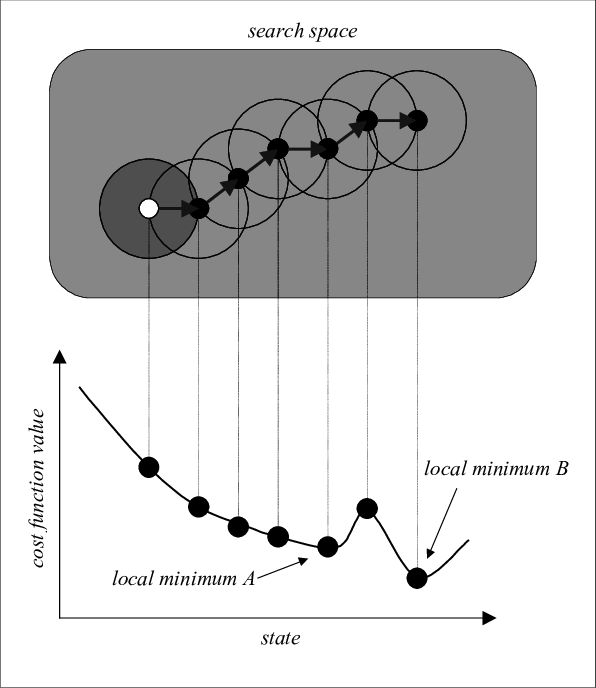
\includegraphics[]{images/metaheuristics.png}
    \caption{General behavior of a metaheuristic method}
    \label{fig:metaheur}
\end{figure}

Metaheuristic methods can be classified into two main categories: single-solution and population-based methods. Single-solution methods start with an initial solution and iteratively improve it by applying a set of moves or transformations. The single-solution metaheuristics that we implemented are Variable Neighborhood Search (VNS), Tabu Search and Simulated Annealing. Population-based methods maintain a population of candidate solutions and explore the search space by iteratively generating new solutions through genetic operators such as crossover and mutation. For the population-based methods we implemented a Genetic Algorithm.





\section{Variable Neighborhood Search}
The Variable Neighborhood Search (VNS), proposed by Mladenović and Hansen in 1997,  is a metaheuristic optimization algorithm used to solve combinatorial optimization problems. The basic idea of VNS is to iteratively apply a perturbation operator to the current solution and then perform a local search around the perturbed solution. VNS is known for its flexibility and ability to escape from local optima by exploring different neighborhood structures.

In our implementation the VNS algorithm tries to improve the solution made by the 2-opt algorithm. In order to try to escape from the local minima produced by the 2-opt, the algorithm performs a random swap of 5 edges (called kick), see Figure \ref{fig:VNS} %%%


\begin{figure}[!h]
    \centering
    \begin{tikzpicture}
        \tikzstyle{city} = [fill=purple!20,rounded corners]
    

        \filldraw[color=blue!60, fill=blue!5, very thick](0,0) circle (4);

        \filldraw[color=red!60, fill=red!5, very thick](0,0) circle (1.5);

        \filldraw[color=red!60, fill=red!5, very thick, fill opacity=0.2](-2.5,-2) circle (1.5);

        
       
        \node[city,label=above:$x^{(n)}$] (A) at (0,0){};
        \node[city] (B) at (-2.5,-2){};

        

        \draw[->] (A) edge[bend right] node [right] {} (B);

        

        


        % define a random point (C) on this circle
        \path (0,0) ++(-45:1.5) coordinate (C);

        % draw (C) with a label
        \fill[black] (C) circle[radius=2pt] ++(1.5:1em) node {2opt};

        % define a random point (D) on this circle
        \path (0,0) ++(40:4) coordinate (D);

        % draw (C) with a label
        \fill[black] (D) circle[radius=2pt] ++(4:1em) node {3opt};
        

        \draw[dashed] (A) -- (C);
        \draw[dashed] (A) -- (D);




        %\draw[->] (0,0) arc (0:200:1.5);
       
    
    \end{tikzpicture}
    \caption{Example of VNS kick} \label{fig:VNS}
\end{figure}



Then it reapplies the 2-opt procedure and if it finds a better solution cost, it updates the global solution.
The overall procedure of Algorithm \ref{algo:VNS} is applied until a certain time limit is reached.
The algorithm requires $O(n)$ time for each kick, because after the swap operation we have to update the structure that contains all the nodes of the graph. We also have to sum the time required by the 2-opt algorithm. This time at the end has to be multiplied by the number of iterations that this procedure is performed. 

\begin{algorithm}[h!]
    \caption{VNS}\label{algo:VNS}
    \begin{algorithmic}[1]
    \Require $G = (V,E), c:E \to \mathbb{R}^+$
    \Ensure $\text{sub optimal TSP solution}$


    \State $solution \gets$ 2OPT(G)
   
   
    \While{$ !time\textunderscore expired$}
    \State kick(solution)   
    \State $ solution \gets $ 2OPT(solution)
    
    
    \If{cost(solution) < cost(best\textunderscore solution)}
    \State $ best\textunderscore solution \gets$ solution
    \EndIf
    

    \EndWhile

    \end{algorithmic}
\end{algorithm}

\subsection{Tuning of VNS}

\begin{figure}[!h]
    \centering
    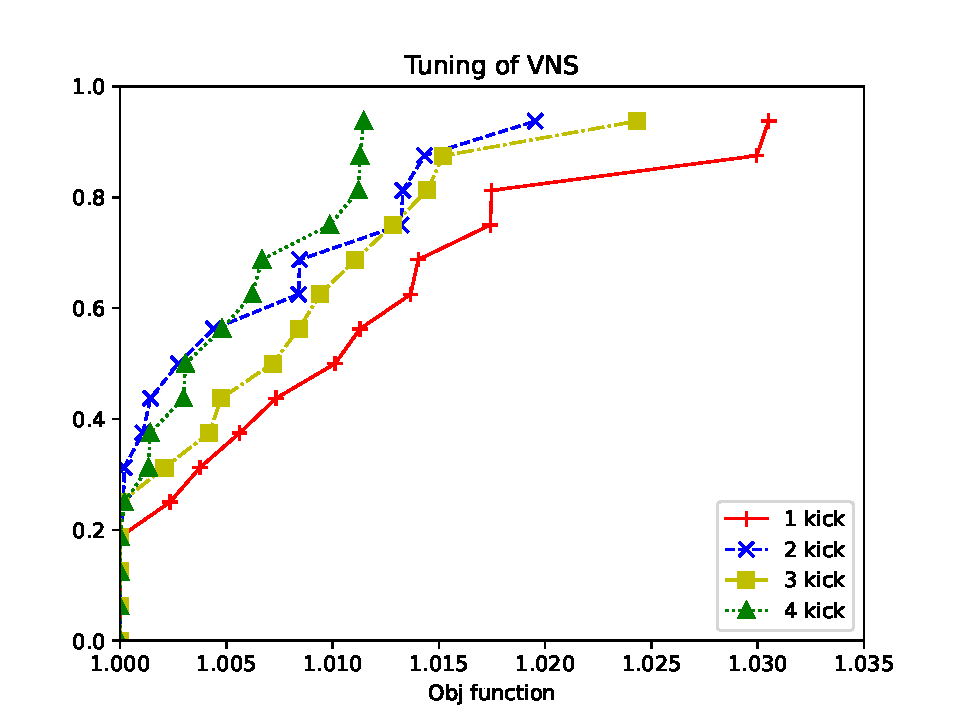
\includegraphics[width=\textwidth]{images/vns.pdf}
    \caption{VNS Tuning of number of kicks}
    \label{fig:vns}
\end{figure}

The VNS algorithm can vary its efficiency depending on how many kicks it computes at each iteration.

After some tests we noticed that the size of the instance didn't really affected the decision of how many kicks to make, so we made a comparison using the same number of kicks for each instance, disregarding its actual size, see Figure \ref{fig:vns}.





\section{Tabu Search}
Tabu search is a metaheuristic method created by Fred W. Glover in 1986.
It is based over the concept of "tabu" which means "prohibited" or "forbidden", following the idea that that the algorithm actually maintains a tabu list that keeps track of recent moves that are prohibited from being repeated. 
Tabu search is known for its ability to find good-quality solutions in a relatively short amount of time, although, as all other heuristic methods, it does not guarantee finding the optimal solution.

The algorithm \ref{algo:tabu} starts with an initial solution, which can be generated randomly or by using a construction heuristic. In our implementation the initial solution is generated by the Greedy heuristic with the GRASP multistart variant, and optimized using the 2-opt algorithm.

At every iteration of the tabu algorithm, we select the pair of edges that have the minimum value of $\Delta$ (defined as in 2-opt, see Equation \ref{eq:delta}). Unike 2-opt algorithm, in Tabu Search doesn't matter if delta is negative or positive, we only take the minimum computed delta of the nodes that are not marked as “tabu” and then we select those nodes as candidate for a swap of edges (as in Figure\ref{fig:2OPT}).  After every swap, one of the four nodes involved is randomly select, and it is inserted into the “tabu” list.

The practice of using and updating a "tabu" list is used to prevent cycling, which means repeatedly visiting the same solutions over and over, without actually improving the current local optima. This allows the tabu method to diversify the search and explore different regions of the solution space. Thanks to this feature the algorithm moves around the solution space avoiding being stuck in local optima, and trying to find a better solution value, as can be seen in Figure \ref{fig:TABU}. This property can also be seen in practice, as in Figure \ref{fig:TABUPERF} where it is shown the possible output costs of the different solutions found by Tabu Search at each iteration.

\begin{figure}[!h]
    \centering
    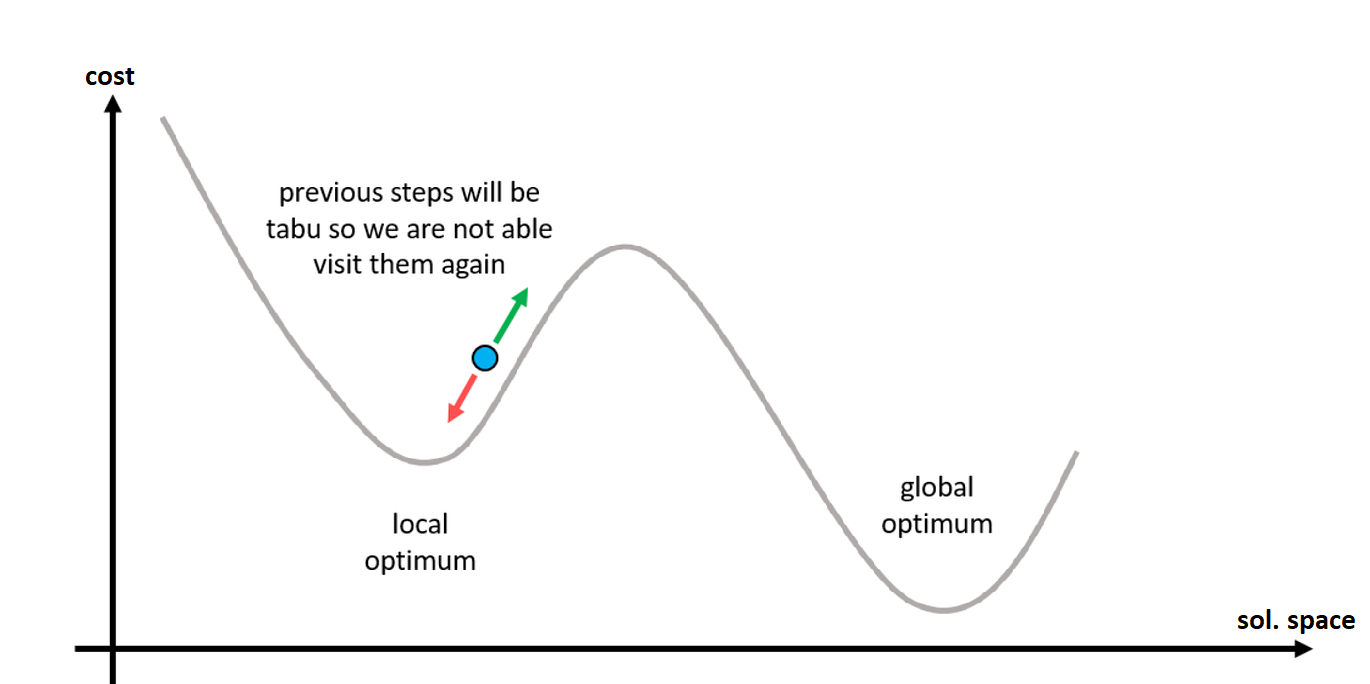
\includegraphics[width = \textwidth]{images/tabu.png}
    \caption{General behavior of a TABU method}
    \label{fig:TABU}
\end{figure}

\begin{figure}[!h]
    \centering
    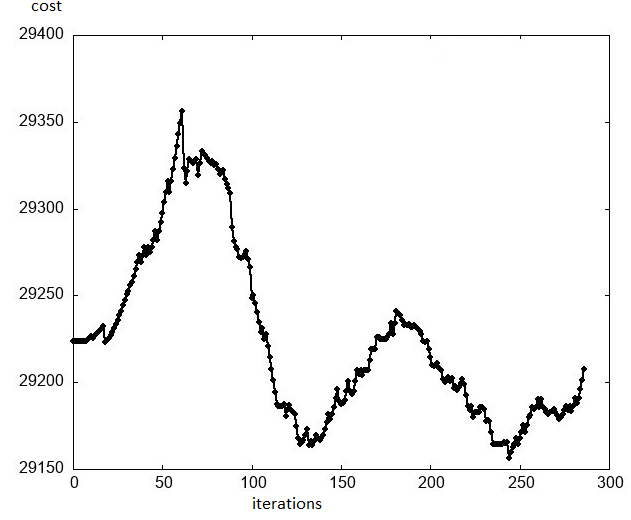
\includegraphics[scale=0.8]{images/tabuperf.png}
    \caption{progress of the objective function of tabu}
    \label{fig:TABUPERF}
\end{figure}

In order to implement the tabu list we create a list of length equals to the number of the nodes of the graph. Every time a node is selected to be a “tabu node” we set its corresponding element of the list equals to the number of the current iteration. Then this node cannot be involved in any swap operations until the number of the next iterations have overcome the value of a parameter called \textit{Tabu Tenure} that we saved as $T_{max}$, representing the number of iterations a node is forced to remain a "tabu" node and cannot be selected in a swap operation.
The value of $T_{max}$ is equivalent to the minimum between a \textit{Tabu Tenure} value and the number of nodes divided by the \textit{Tenure Ratio}, assuring that there are always nodes not labeled as forbidden and that can be used in the swap operation.

Each swap requires time equal to $O(n)$ to rearrange the array containing the actual solution.
The algorithm stops after a given time limit returning in output the best solution found until then.

\begin{algorithm}[!h]
    \caption{Tabu}\label{algo:tabu}
    \begin{algorithmic}[1]
    \Require $G = (V,E), c:E \to \mathbb{R}^+$
    \Ensure $\text{sub optimal TSP solution}$


    \State $solution \gets$ 2OPT()
    \State $cost \gets$ cost\textunderscore 2OPT()
    \While{$ !time\textunderscore expired  $}
    \State $\Delta\gets$ $*$ best delta among all pairs of nodes that are not in the tabu list $*$
    \State $*$ choose a random node of delta and insert it into tabu list $*$
    \State $*$ updates tabu list $*$
    \State $edge\textunderscore 1 \gets$ new edge (a,b) that has to be inserted
    \State $edge\textunderscore 2 \gets$ new edge (b',a') that has to be inserted
    \State $swap(edge\textunderscore 1,edge\textunderscore 2) $
    \State $cost += \Delta$

    \If{cost < cost(best\textunderscore solution)}
    \State $ best\textunderscore solution \gets$ solution
    \State $ cost(best\textunderscore solution) \gets$ cost
    \EndIf
    

    \EndWhile

    \end{algorithmic}
\end{algorithm}



\begin{figure}[!h]
    \centering
    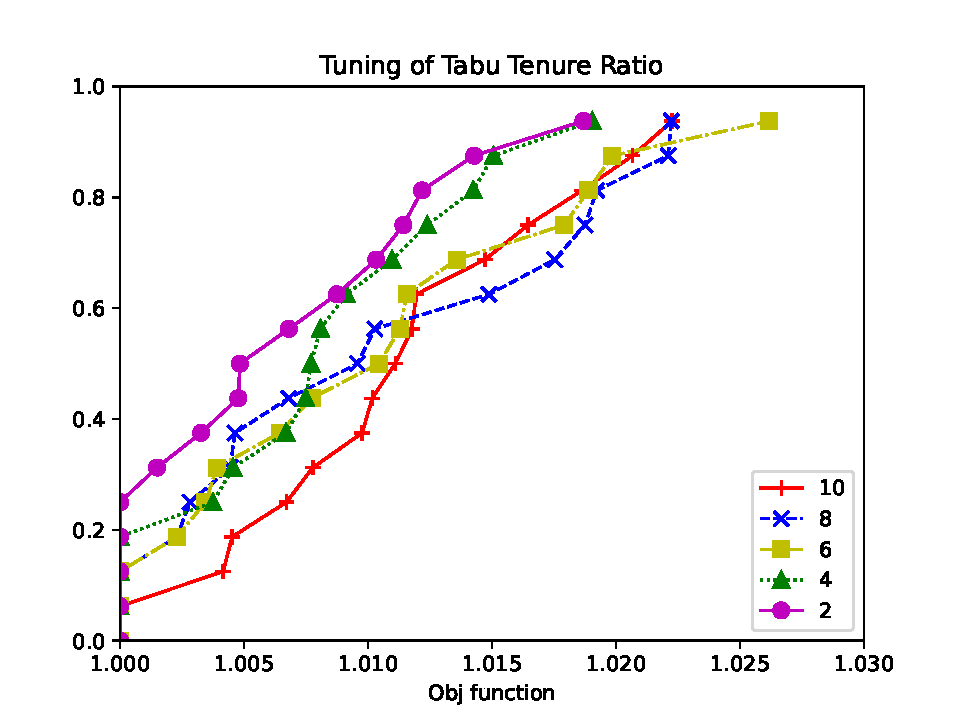
\includegraphics[width=\textwidth]{images/tabu.pdf}
    \caption{Tuning of Tabu Tenure Ratio}
    \label{fig:tabu}
\end{figure}
\subsection{Tuning of Tabu}

This section is used to identify and then tune the possible parameters that can alter the results of the Tabu Search algorithm.



The first parameter we tested is the \textit{Tenure Ratio}, a value that in our implementation serves the role of choosing the right \textit{Tenure} (or $T_{max}$) depending on the size of the input instance.

In Figure \ref{fig:tabu} we can see that a \textit{Tenure Ratio} of 2 has to be chosen to obtain the best performance on all the instances used.



The secondo parameter to be tested is the \textit{Tenure} itself. As an initial hypothesis we thought that having a bigger \textit{Tenure}, in the sense of forbidding certain moves for more time, could end up in finding better solutions, but Figure \ref{fig:tabu2} actually shows the opposite.

\begin{figure}[!h]
    \centering
    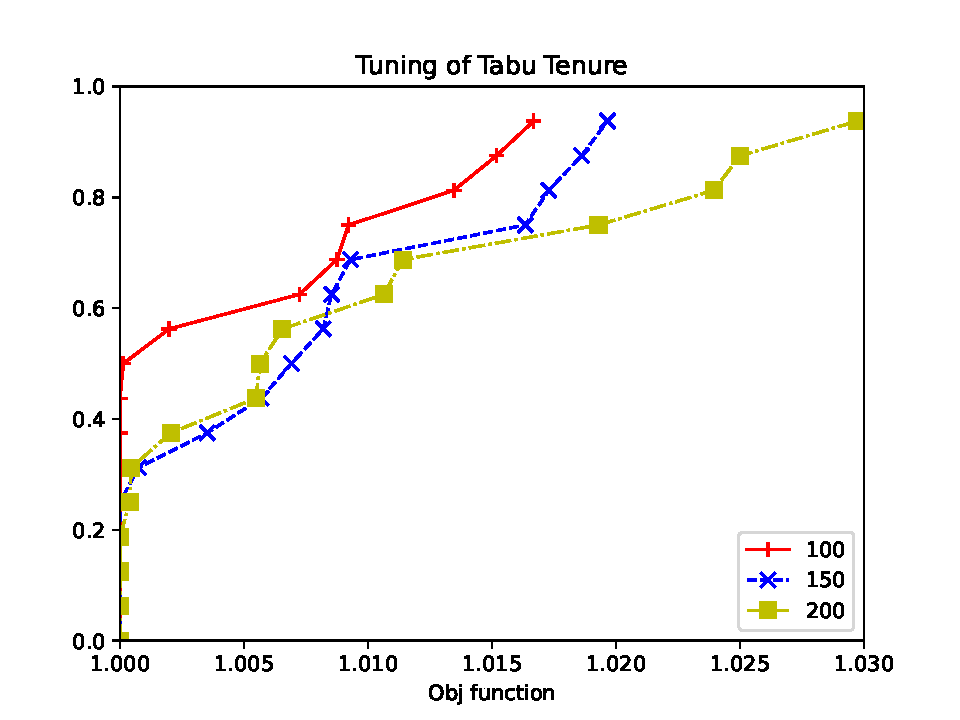
\includegraphics[width=\textwidth]{images/tabu2.pdf}
    \caption{Tuning of Tabu Tenure}
    \label{fig:tabu2}
\end{figure}


\section{Simulated Annealing}

Simulated annealing is a metaheuristic optimization algorithm that can be used to solve the Travelling Salesman Problem (TSP).
The name of the algorithm comes from annealing in metallurgy, a technique involving heating and controlled cooling of a material to alter its physical properties. This method uses a probabilistic technique that usually archives an approximate solution of the global minimum.

Just like other metaheuristics, this algorithm starts with an initial solution, which can be generated randomly or using a heuristic. In our implementation we use the output of the Greedy heuristic with the GRASP and multistart variant as the initial solution that we want to improve.

At each iteration of the Algorithm \ref{algo:SimulatedAnnealing}, we select two edges $(a,a')$,$(b,b')$ randomly, where $a,a',b$ and $b'$ are distinct nodes and compute the $\Delta$ as in Equation \ref{eq:delta}. If there would be an improvement over the current solution, we swap the edges (as in Figure\ref{fig:2OPT} ). Else if the swap would result in the worsening of the solution, there is still a certain probability of making the swap anyway depending on a probability function over a parameter called Temperature. \\The probability function used is defined as:



\begin{equation*}
    e^{\frac{-\Delta \operatorname{c}(a,b)}{T}}
\end{equation*}

\begin{algorithm}[!h]
    \caption{Simulated annealing}\label{algo:SimulatedAnnealing}
    \begin{algorithmic}[1]
    \Require $G = (V,E), c:E \to \mathbb{R}^+$, a valid tour solution
    \Ensure $\text{sub optimal TSP solution}$

    \State cost $\gets$ cost(solution)

    \State $T \gets   T_0 $
    \State $ \alpha \gets  0.95 $
    \State $ iter \gets  0 $
   




    \While{$ !time\textunderscore expired$}
    

    \State $*$ Select two random edges and apply 2OPT move $*$

    
    \State $\Delta \gets *$ Difference of cost due to the 2OPT move $*$  
    
    
    \If{$\Delta \leq 0$}
    \State $*$ Update solution $*$
    \State cost $\gets$ cost + $\Delta$
    \Else 
    \State $*$ Update solution with probability $ e^{-\Delta \over T}*$

    \EndIf

    \State $T \gets T \cdot \alpha$
    \State $iter++ $
    \If{ $iter \geq$ 100}
    \State $T \gets   T_0$
    \State $iter \gets  $ 0
    \EndIf
    

    \EndWhile

    \end{algorithmic}
\end{algorithm}

where $T$ is called \textit{Temperature} and is computed over time as $T = \alpha \cdot T$, with $\alpha$ called \textit{cooling parameter} and starting with $T = T_0$ that actually depends on the input.

In our implementation of Algorithm \ref{algo:SimulatedAnnealing} the initial value for the temperature $T_0$ is equal to the cost of the input solution found by the GRASP Algorithm, divided by the number of nodes of the instance of the current TSP problem. Then at each iteration, $T$ is multiplied by the cooling parameter $\alpha$. After 100 iterations of the algorithm, the temperature is newly set to its initial value $T_0$.

Each swap requires time equal to $O(n)$ to rearrange the array containing the actual solution.
The algorithm stops its iteration after a given time limit.

	


\subsection{Tuning of Simulated Annealing}

To tune the probability used in the Simulated Annealing algorithm, the parameter to test is the \textit{cooling parameter} $\alpha$. Starting from the value of 0.99, we tested the range [0.95,0.99] to not have a too big decrease of $T$ at each iteration.

We can see in Figure \ref{fig:sa} that $\alpha = 0.95$ wins over the other values, for the only exception of $\alpha = 0.96$ in the higher percentiles.

\begin{figure}[!h]
    \centering
    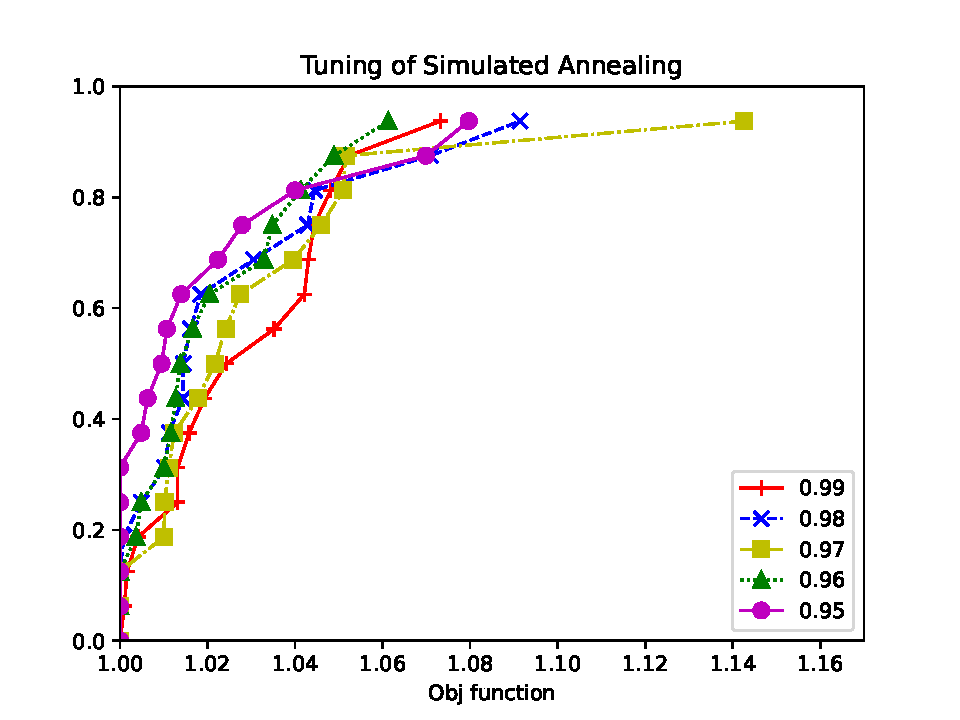
\includegraphics[width=\textwidth]{images/sa.pdf}
    \caption{Tuning of Simulated Annealing}
    \label{fig:sa}
\end{figure}

\section{Genetic Algorithm}
Another approach to solving the TSP is to use a Genetic Algorithm, which is a type of heuristic optimization algorithm inspired by the process of natural selection. Genetic algorithms work by creating an initial population of candidate solutions (called chromosomes), and then repeatedly applying genetic operators such as crossover and mutation to generate new, potentially better solutions, called offspring [\ref{algo:genetic}].


The choices of crossover and the chromosomes that make it to the next generation are based on the fitness of each chromosome, that is defined as minus the cost of the tsp tour. The Genetic Algorithm then selects the fittest individuals to serve as parents for the next generation, with the hope that their good qualities will be passed on to their offspring.

To add some randomness in the hope of escaping the local optimums, a mutant is added with some probability to each new generation. A mutant is a chromosome of the current generation, chosen at random, to which a mutation has been applied, aka has some edges swapped at random.

Through this iterative process, the Genetic Algorithm explores the space of possible solutions and gradually converges on a near-optimal tour.

In conclusion, the Genetic Algorithm is a powerful and flexible approach to solving the Travelling Salesman Problem. While it may not always find the optimal solution, it can quickly find high-quality solutions that are good enough for many practical applications.

\begin{algorithm}
    \caption{Genetic algorithm}\label{algo:genetic}
    \begin{algorithmic}[1]
    \Require $G = (V,E), c:E \to \mathbb{R}^+$
    \Ensure $\text{sub optimal TSP solution}$
    
    \State $population \gets *$ initialize population of chromosomes using GRASP $*$

    \State $ generation \gets 0$

    \While{$generation < MAX \textunderscore GENERATION$}

        \State $parents \gets *$ initialize the offsparents  using a selection algorithm$*$
        \State $offspring \gets *$ initialize the offspring using crossover $*$

        \State $mutant \gets *$ if appropriate, initialize the mutant $*$

        \State $ newGeneration() $
        \State $ generation++ $

    \EndWhile

    \State $ solution \gets *$ chromosome with best fitness$*$

    

    \end{algorithmic}
\end{algorithm}

It's important to state elitism is implemented which means that the chromosomes with higher fitness (aka with lower cost) are always passed down to the next generation, ensuring that the best solution within all iterations of the Genetic Algorithm is never killed. 

\subsubsection{Implementation choices}
There are several algorithms that can be used in conjunction with Genetic Algorithm to enhance its performance.
During each iteration of the Genetic Algorithm, selection, crossover and mutation are the main steps to compute to produce the new generation.
Selection algorithm determine which individuals from the current population should be chosen for reproduction to generate the next generation. The most commonly used selection algorithms are:

\begin{itemize}
    \item Roulette Wheel Selection: each chromosome in the population is assigned a probability of selection based on its fitness. The probabilities are proportional to the fitness of the individual, so that individuals with higher fitness have a higher chance of being selected. A random number is then generated, and the individual corresponding to the selected probability is chosen for reproduction. (It is the algorithm that we chose to implement in our project)
    \item Tournament Selection: a small subset of the population is randomly selected, and the individual with the highest fitness within that subset is chosen for reproduction.
\end{itemize}

After choosing two parents using selection, a new individual must be generated using a crossover algorithm. 
These algorithms determine how the tour information is exchanged between two parents during reproduction. Common crossover algorithms include single-point crossover, two-point crossover, and uniform crossover.
We implemented the single-point crossover and it works by choosing a single breaking point at random within the solutions of the parents and generating a partial new solution merging the chosen halves from the parents, without inserting duplicate nodes.
After that the new solution must be repaired and we chose to do so using the \ref{extramileage} Extra-Mileage Algorithm.

Mutation is computed within a certain probability and the chosen individual has its tour modified by the swapping of two random edges. Other common mutation algorithms include bit-flip mutation and inversion mutation.


\begin{figure}[!h]
    \centering
        %Prima riga
        \begin{subfigure}{0.48\textwidth} %Controllo della posizione in orizzontale
            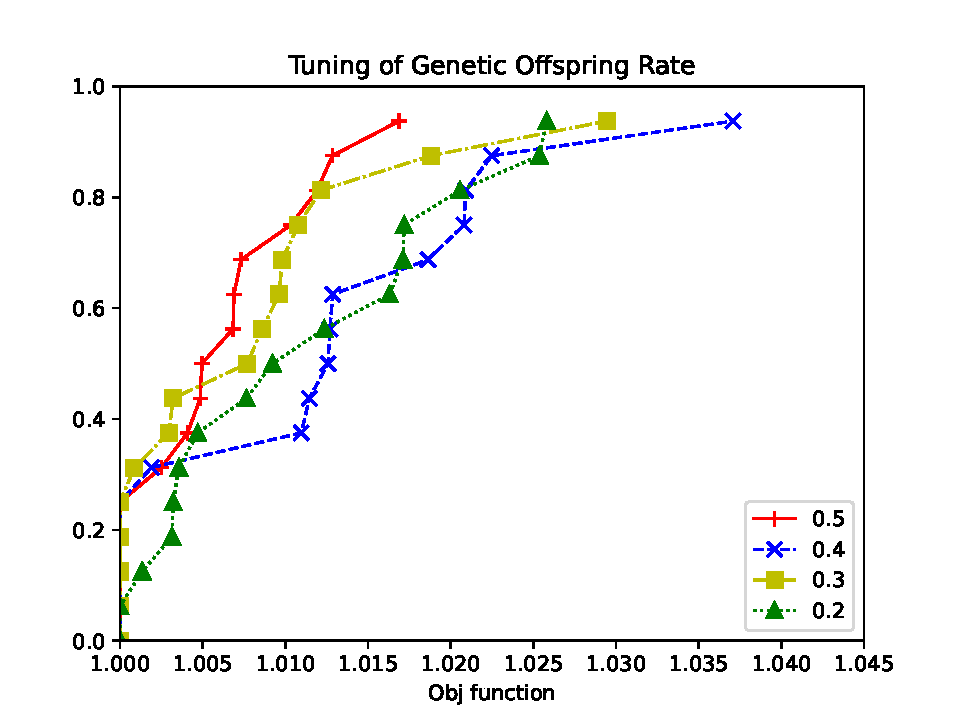
\includegraphics[scale=0.45]{images/genoff.pdf} 
            \caption{Tuning of Offspring Rate}
            \label{fig:genoff}
        \end{subfigure}
        \begin{subfigure}{0.48\textwidth}
            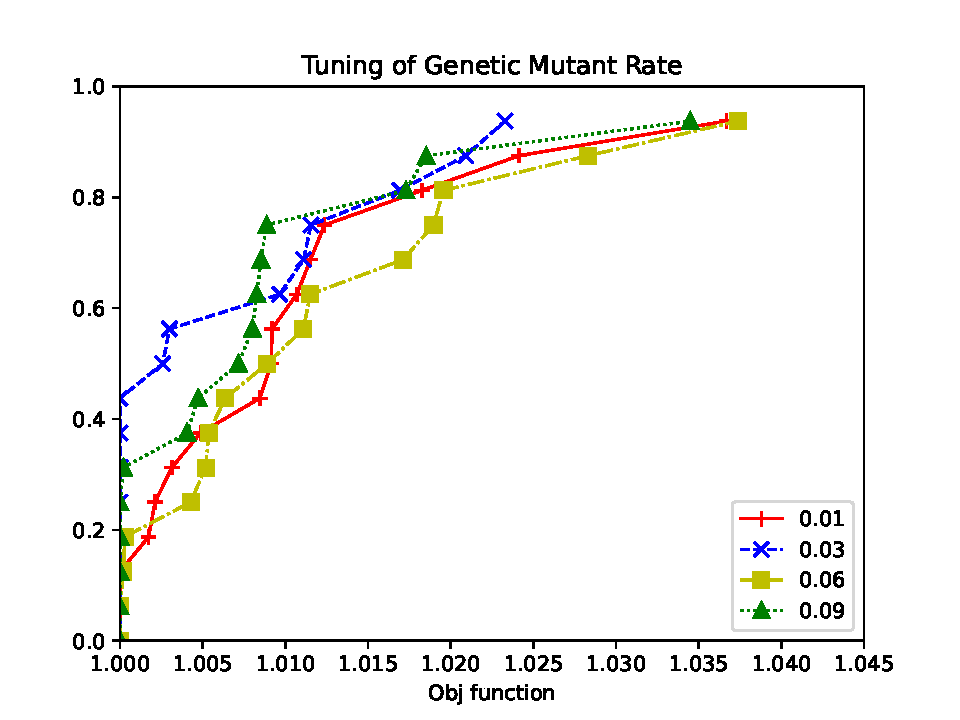
\includegraphics[scale=0.45]{images/genmut.pdf}
            \caption{Tuning of Mutant Rate}
            \label{fig:genmut}
        \end{subfigure}
    \caption{Tuning of the Genetic algorithm}
    \end{figure}

\subsection{Tuning of Genetic}

The most important parameters in the Genetic algorithm are the \textit{Offspring Rate} and the \textit{Mutant Rate}.

The \textit{Offspring Rate} determines the size of the new offspring generation based over a percentage of the size of the actual generation. This value changes the rate of finding possible better chromosomes, slowling or speeding up the process of natural selection.

In Figure \ref*{fig:genoff} can be seen that the values that compete the most are 0.5 and 0.3, but in the final implementation of the algorithm we chose \textit{Offspring Rate} = 0.5 since it performed better in the most cases.


The \textit{Mutant Rate} is tuned to add some well weighted randomness to the algorithm. Too many mutants can lead to worse possibilities of improvement, but a mutant is essential to assert a possibility of escapism from a possible local optima. 

We tested the range [0.1,0.9] to keep the probability of adding a mutant really low, and we can see in Figure \ref*{fig:genmut} that both 0.03 and 0.09 compete really well, but we chose to use a \textit{Mutant Rate} = 0.09.





\section{Comparison of Metaheuristic Algorithms}
This section is dedicated to the comparison of the Metaheuristic algorithms described above. 
It is important to highlight that these algorithms can vary its performance depending on their implementation, thus the results we are going to describe are intrinsically correct only within the boundaries of our own model.

In Figure \ref{fig:meta} we are comparing Tabu Search, VNS, Genetic and Simulated Annealing over the same instances, within the same time limit of 5 minutes, all of them with their corresponding tuned parameter, to assert the best possible performance.



\begin{figure}[!h]
    \centering
    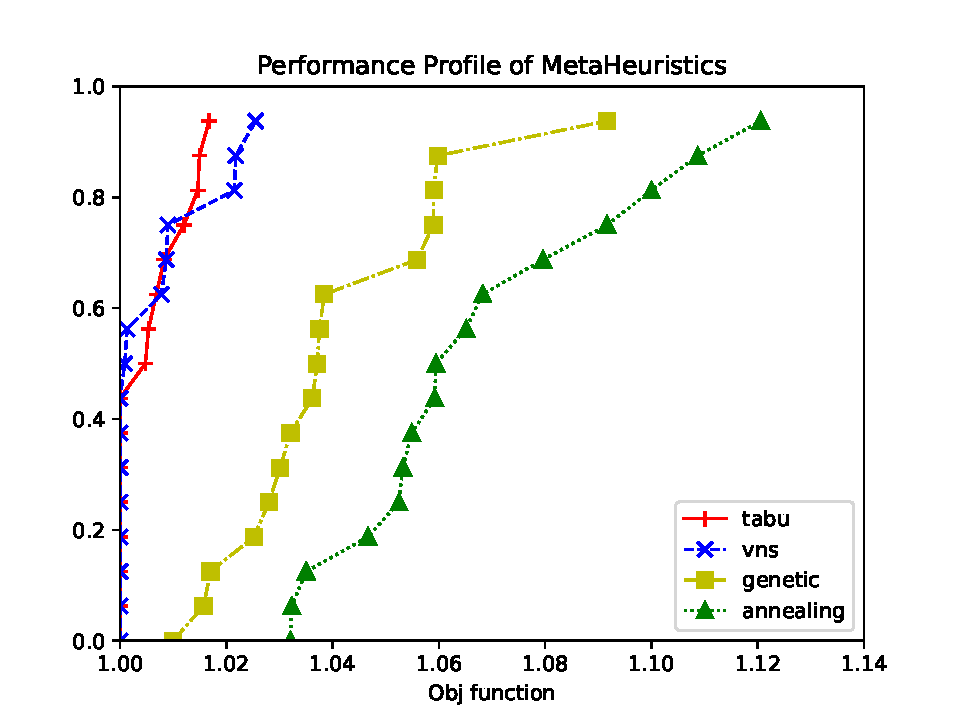
\includegraphics[width=\textwidth]{images/meta.pdf}
    \caption{Performance Profile of Metaheuristic algorithms}
    \label{fig:meta}
\end{figure}

\begin{table}[]
    \centering
    \begin{tabular}{lcccc}
    \cline{2-5}
                & \textbf{Tabu}   & \textbf{VNS}    & \textbf{Genetic} & \textbf{S. Annealing} \\ \hline
    att48.tsp   & 10611.110112    & 10625.430487    & 10995.308862     & 10983.016723       \\
    att532.tsp  & 29019.678235    & 28600.917059    & 30289.711639     & 29936.067989       \\
    d493.tsp    & 36979.874325    & 36370.285809    & 37735.484078     & 37545.598513       \\
    d657.tsp    & 51384.866148    & 50962.833321    & 54008.992502     & 54281.845932       \\
    dsj1000.tsp & 19803626.0 & 19821191.0 & 20114713.0  & 21618389.0  \\
    lin318.tsp  & 43502.354696    & 43270.515360    & 44658.919744     & 45646.363287       \\
    p654.tsp    & 34995.096723    & 35309.748105    & 35591.094654     & 39214.526200       \\
    pcb442.tsp  & 52965.274330    & 53426.635390    & 54301.288319     & 55783.711331       \\
    pr1002.tsp  & 268635.034053   & 274412.315655   & 293234.499257    & 295497.542051      \\
    pr439.tsp   & 110930.029029   & 109612.967166   & 112684.510372    & 118337.491854      \\
    rat575.tsp  & 7031.068022     & 7210.570174     & 7446.014269      & 7447.548178        \\
    rat783.tsp  & 9267.450174     & 9339.766424     & 9785.356566      & 9753.999949        \\
    rd400.tsp   & 16154.800276    & 16044.900084    & 16205.288761     & 16559.390143       \\
    u574.tsp    & 38885.965904    & 38700.991445    & 40137.238017     & 41341.810322       \\
    u724.tsp    & 44654.674979    & 43996.953223    & 45323.345043     & 46611.944462       \\
    vm1084.tsp  & 250014.164445   & 255459.278942   & 259630.598039    & 277195.165549      \\ \hline
    \end{tabular}
    \caption{Results of Metaheuristic Methods}
    \label{table:meta}
    \end{table}

    Data in Table \ref{table:meta} show the resulting values found running the Metaheuristic Algorithms over the relative instances. We can see that Tabu Search and VNS perform both really well, with Tabu being a little more precise over bigger instances. 








 

\clearpage{\pagestyle{plain}\cleardoublepage} 
\chapter{Exact Algorithms} 
\label{chapter:exact} 
Exact algorithms for the TSP are methods that guarantee finding the optimal solution to the problem by exploring all possible combinations of city tours. These algorithms are based on exhaustive search and systematic enumeration, ensuring that no potential solution is overlooked. While they may work well for small instances of the TSP, they become computationally infeasible for larger problem sizes since it leads to a time complexity of $O(n!)$.


\section{Benders}
Benders' Decomposition is a powerful optimization technique used to solve large-scale combinatorial problems like the Traveling Salesman Problem (TSP). It was introduced by Jacques F. Benders in the 1960s and has since become a widely used approach in the field of mathematical programming.

The Traveling Salesman Problem is known to be a challenging NP-hard problem, meaning that finding the optimal solution for large instances can be computationally intractable using traditional methods like brute-force or exact algorithms. Benders' Decomposition addresses this issue by breaking down the problem into smaller, more manageable subproblems and solving them iteratively.

The basic idea behind Benders' Decomposition is to partition the original problem into a master problem and multiple subproblems. The master problem is an integer linear programming (ILP) relaxation of the original TSP, allowing for the relaxation of some constraints. It aims to find a lower bound on the optimal solution value of the TSP. The subproblems, also known as \textit{Benders' cuts} or \textit{feasibility cuts}, are used to correct the solution obtained from the master problem by adding additional constraints that remove infeasible solutions, called \textit{Subtour Elimination Constraint} (SEC).

\begin{equation*}
    \sum_{e \in E(S_k)} x_e \leq |S_k|-1 \quad \quad \forall S_k: k=1,2,...
\end{equation*}

In our implementation \ref{algo:benders} we use CPLEX to build an initial ILP model of the TSP instance with only the degree equals 2 constraints for each node. We solve this model iteratively to obtain a solution,  which may not be feasible for the original TSP, in the sense that it contains subtours (internal cycles). Each subtour is considered a connected component and we generate Benders' cuts based on these components to eliminate them from consideration in subsequent iterations of the algorithm. We add these cuts to the CPLEX model, called \textit{Subtour Elimination Constraint} (SEC), which tightens the relaxation and improves the solution quality.



\begin{algorithm}
    \caption{Benders Algorithm}\label{algo:benders}
    \begin{algorithmic}[1]
    \Require $G = (V,E), c:E \to \mathbb{R}^+$
    \Ensure $\text{Optimal TSP solution}$
    
    \State $*$ initialize a basic CPLEX model with degree constraints $*$

    \State $ ncomp \gets 0$

    \While{$ !time_{expired} $}

        \State $*$ Solve CPLEX model$*$
        \State $ncomp \gets $ number of connected components

        \If{$ncomp = 1$}
            \State $*$ we found the optimal solution $*$
            \State \Return Solution
        \EndIf

        \State $*$ computes Patching Heuristic $*$

        \ForEach{connected component}

        \State $*$ add SEC $*$

        \EndFor

       

    \EndWhile

    \State \Return best Solution found


    \end{algorithmic}
\end{algorithm}

\subsection{Patching Heuristic}
In the Algorithm \ref{algo:benders} at line 10, we compute the Patching Heuristic.
It is an extension of Benders' Decomposition that aims to improve the quality of solutions obtained by the original Benders' algorithm before it terminates. 

It addresses a limitation of Benders' Decomposition, which may produce solutions with a relatively large optimality gap due to the relaxation of the TSP constraints in the master problem. The patching heuristic helps close this gap by iteratively improving the solution through additional modifications.

At each iteration of Benders, a solution is obtained, but it might still contain subtours due to the relaxation of constraints. The Patching Heuristic aims to identify and remove these subtours from the solution, thus achieving a feasible solution with tighter bound on the optimal solution value.

In our implementation, the Patching Heuristic repairs the current solution with subtours one component at a time until all components are connected. 
Starting from component number 1, it tries to find the edge that connect this component to a different one with lowest $\Delta$ (as defined in Equation \ref{eq:delta}) and then merges the two components. This process is repeated until all components are merged into one.

\begin{figure}[!h]
    \centering
    \begin{tikzpicture}
        \tikzstyle{city} = [fill=purple!20,rounded corners]


        \node[city] (A) at (2.3,5.0){};
        \node[city] (B) at (2.6,6.5){};
        \node[city] (C) at (7.7,5.5){};
        \node[city] (D) at (6.7,4.5){};
        \node[city] (E) at (3.0,4.0){};
        \node[city] (F) at (3.5,6.5){};
        \node[city] (G) at (4.6,5.5){};
        \node[city] (H) at (6.5,6){};


        %\draw[->] (C.west) -- (E.east);
        %\draw[->] (B.south) -- (A.east);
        \draw[] (C) edge (D) (E) edge (A) (A) edge (B) (B) edge (F) (F) edge (G) (G) edge (E) (D) edge (H) (H) edge (C);

        \draw[dashed, red] (D) edge (E) (H) edge (G);

    \end{tikzpicture}
    \caption{Example of Patching Heuristic} \label{fig:patch}
\end{figure}




\section{Callback For SECs}

A TSP problem can also be solved by the branch and cut technique with the help of CPLEX callback functions. Branch and cut combines the concepts of branch and bound with cutting planes to efficiently explore the solution space and find optimal solutions. The branch and cut method begins by solving a relaxation of the original problem. This relaxation (known as LP relaxation) allows fractional solutions, which are not feasible for the original problem, but it provides an upper bound on the optimal solution value.
Next, the algorithm branches on the fractional variables in the LP relaxation, creating multiple subproblems, and then solves each subproblem separately.\\
To speed up the search the method uses valid inequalities (cutting planes) that can be added to the LP relaxation to eliminate fractional solutions, with the result of improving the lower bound on the optimal solution. \\
The branch and cut algorithm iteratively performs branching, solving LP relaxations, and adding cutting planes until it either finds an optimal solution or proves that no better solution can be found. \\
The CPLEX software can invoke a custom callback function whenever a new integer solution is found during the process of searching for a new solution .This solution takes the name of the candidate solution.\\
In this case we check if the solution provided by CPLEX is feasible. In this case we are checking if it contains subtours. If the answer is positive, we add SECs for the connected component. \\
The main difference between this approach and Bender’s method is that in this case only a single decision tree is generated.

\begin{algorithm}
    \caption{Callback For SECs}\label{algo:SECcallback}
    \begin{algorithmic}[1]
    \Require TSP solution with subtours
    \State find subtours that belong to the solution
    \ForEach {subtour s$\in$ solution}
    \State add SEC that remove subtour s
    \EndFor
    
    \end{algorithmic}
\end{algorithm}


\section{User Cuts Callback}
This time we present another possible implementation of a CPLEX callback. Now the callback is used in the relaxed solution of the problem. This special type of solution doesn’t consider the integer constraints of the decision variables. \\
The task that this specific callback has to solve is the same as the one presented in the previous section, but the function  is applied on the continuous relaxation of the problem.\\
In order to implement this type of procedure we need the use of the Concorde library, because the solution found is not integer.
We use the function \textit{CCcut\_connect\_components} to find the number of connected components in a fractional solution. Now if there is only one component, it may not be a TSP solution, because it could be still fractional. In this case we use the function \textit{CCcut\_violated\_cuts} in order to cut this solution.\\


\subsection{Tuning of User Cuts Callback}
We cannot apply this type of callback at every node of the branching tree, because it would take too much time to find the solution, due to the high time taken by the algorithms present in the concorde library. So we apply this procedure only if the “number” that identify every node of the branching tree has a particular feature.
Thus the parameter to tune is strictly connected to how many nodes of the branching tree can have the callback applied to.
In Figure \ref{fig:concorde} the numbers tested refer to the ratio of nodes to which the callback is applied. A value of 2 refers to half the nodes, while a value of 10 refers to a tenth of the nodes and so on.

\begin{figure}[!h]
    \centering
    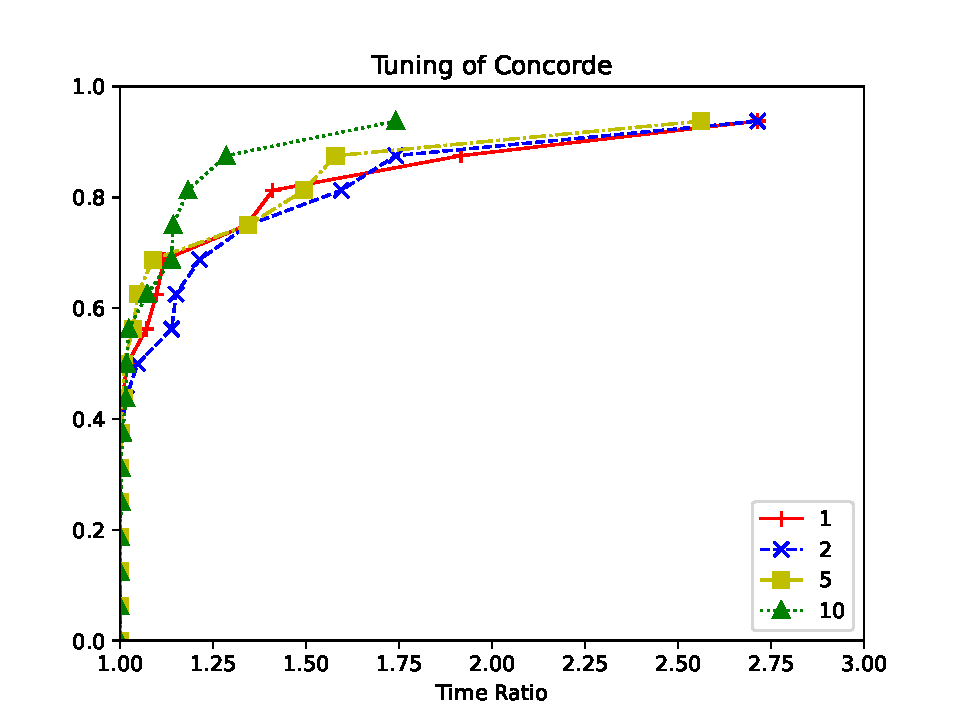
\includegraphics[width=\textwidth]{images/concorde.pdf}
    \caption{Tuning of node ratio in User Cuts Callback}
    \label{fig:concorde}
\end{figure}

\section{Comparison of Exact Methods}

We tested the performance of all three exact methods mentioned above, running on the same instances for 5 minutes each. In Figure \ref{fig:exact} it can be seen that all of them performs really well in 30\% of instances, but the User Cuts Callback using the Concorde library actually outperforms the other methods overall, even if it employs time-consuming routines based on Concorde documentation.

It is quite straightforward why Benders Algorithm performs the worst, since it reconstruct the model at each iteration, wasting more time compared to the other methods.

\begin{figure}[!h]
    \centering
    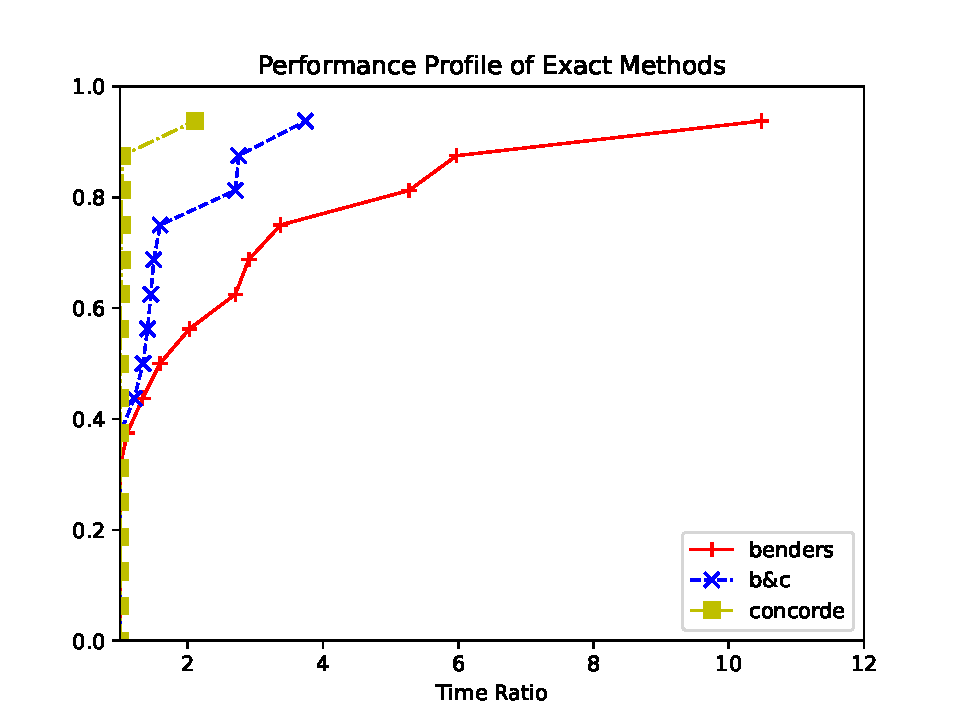
\includegraphics[width=\textwidth]{images/exact.pdf}
    \caption{Performance Profile of Exact Methods}
    \label{fig:exact}
\end{figure}


\clearpage{\pagestyle{plain}\cleardoublepage} 
\chapter{Matheuristics} 
\label{chapter:matheuristics} 
Matheuristics refers to the integration of Mathematical Programming and problem-specific heuristics to develop hybrid algorithms that leverage the strengths of both approaches. Many real-world optimization problems are computationally challenging and may not be efficiently solvable using exact mathematical programming approaches alone. This is where heuristics come into play. Heuristics are approximate methods that trade optimality for computational efficiency. They aim to quickly find good solutions by leveraging problem-specific knowledge, rules of thumb, or iterative improvement techniques.
The combination of mathematical programming and heuristics in matheuristics allows for a powerful approach to tackle complex optimization problems, providing a good balance between solution quality and computational efficiency. It is particularly useful for problems, such as TSP, where finding exact optimal solutions is infeasible or time-consuming, but good-quality solutions are still desired within a reasonable amount of time.
In the following section we present two of such techniques, that are hard fixing and local branching.

\section{Hard Fixing}
Hard-fixing matheuristics is a specific approach that sets the value of certain decision variables to a specific value and then tries to solve the new simplified problem with the remaining variables. By fixing variables, the problem size is reduced, and the solver can focus on finding a solution in a smaller search space.\\
In our case we fix the decision variables that indicate if an edge is selected or not. We fix those variables as selected, and then we try to solve the new problem with the MIP solver.\\
Once the solution is found, the fixed variables are unfixed, and the procedure restarts until a given time limit is reached.
We first find an initial solution to the problem using the greedy heuristic. Then we construct the basic mathematical model, without the SEC. For every edge e that belongs to the solution provided by the heuristic, we choose with a probability equal to \textit{p} $\in$(0,1) if the edge has to be fixed or not. To fix an edge we simply set the lower bound equal to 1 to the variable corresponding to it. At this point the user-cut callback is used to solve the problem.\\ 
Once a solution has been found, all the lower bounds are set to 0, and from this new solution with the same procedure as before new edges are fixed, and so on until the given time limit is reached.\\
The performance of this method is highly conditioned by the type of the initial solution: if the initial solution is not very good, there is the risk that this approach will get stuck on a non-optimal solution.


\begin{algorithm}
    \caption{Hard Fixing}\label{algo:HardFixing}
    \begin{algorithmic}[1]
    \Require $G = (V,E), c:E \to \mathbb{R}^+$
    \Ensure $\text{sub optimal TSP solution}$

    \State $solution \gets$ greedy()
    \State $cost \gets $ cost(solution)
    \State Build basic TSP model in CPLEX



    \While{$ !time\textunderscore expired  $}
    \ForEach {edge e$\in$ solution}
    \State fix e with probability p
    \EndFor
    \State $solution \gets$ findNewSolution()
    \If{cost(solution) < cost(best\textunderscore solution)}
    \State $ best\textunderscore solution \gets$ solution
    \EndIf
    \State unfix all variables
    \EndWhile

    \end{algorithmic}
\end{algorithm}

\subsection{Tuning of HardFixing}
An essential aspect of our hard fixing method's implementation lies in the parameter that governs the probability of fixing a specific edge. Consequently, we have embarked on tuning this parameter to achieve enhanced performance.
\\
Figure \ref{fig:hard} illustrates the diverse probabilities tested in the matheuristic. The values shown in the figure represent the true probabilities divided by ten. Notably, the value 8 demonstrates superior performance, corresponding to selecting 80\% of the edges from the previous solution.
\begin{figure}[!h]
    \centering
    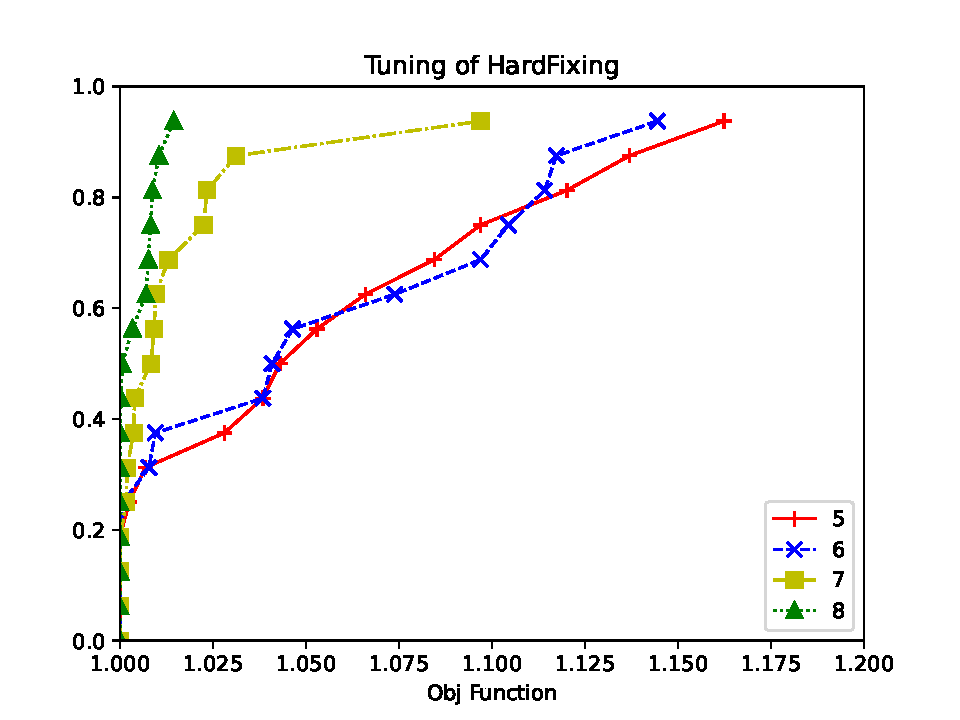
\includegraphics[width=\textwidth]{images/hard.pdf}
    \caption{Tuning of probability in HardFixing}
    \label{fig:hard}
\end{figure}

\section{Local Branching}

The Local Branching or soft fixing, is a matheuristic proposed by M. Fischetti and A. Lodi \cite{fischetti2003local}, that tries to improve the performance of the Hard-fixing matheuristics.\\
A critical point of hard-fixing consists in the choice of the variables that have to be fixed at each step. So, to try to solve this issue, soft fixing requires that a given number of variables have to be fixed, but unlike the hard-fixing method, it doesn’t choose them explicitly. In Local Branching this operation is performed by adding a new constraint that forces the solver to maintain a certain number of variables to the previous value. In our case we add a constraint that informs the solver that a given number of edges have to be maintained. \\

\begin{algorithm}[h!]
    \caption{Local Branching}\label{algo:SoftFixing}
    \begin{algorithmic}[1]
    \Require $G = (V,E), c:E \to \mathbb{R}^+$
    \Ensure $\text{sub optimal TSP solution}$

    \State $solution \gets$ greedy()
    \State $cost \gets $ cost(solution)
    \State Build basic TSP model in CPLEX



    \While{$ !time\textunderscore expired  $}
    \State add constraint \ref{eq:localBranch}
    \State $solution \gets$ findNewSolution()
    \If{cost(solution) < cost(best\textunderscore solution)}
    \State $ best\textunderscore solution \gets$ solution
    \ElsIf{not improvement for a certain number of iteration}
    \State change parameter k
    \EndIf
    \State remove constraint \ref{eq:localBranch}
    \EndWhile

    \end{algorithmic}
\end{algorithm}

The main idea behind this approach is the Hamming distance. This particular distance measures the number of positions at which the corresponding symbols are different. It can be used to calculate the “distance” between two vectors. \\
We can apply this concept to the vector that represents the solution of a TSP instance. This solution can be seen as a binary vector, of length |E|, where each element is set to 1 if the corresponding edge is part of the solution and 0 otherwise. So given two vectors that corresponds to two different solutions of the same TSP instance, the Hamming distance between the two array can be formulated as:
\begin{equation}
   H(x,x^*)= \sum_{e\in E: x_e^*=1}^{}(1-x_e) + \sum_{e\in E: x_e^*=0}^{}x_e
\end{equation}
The first term counts the number of flipped 1’s, and the second counts the number of flipped 0’s. \\
Now looking at the form of the solution provided by the TSP solver, it is possible to add a new constraint that limits the hamming distance between the old and the new solution:

\begin{equation}\label{eq:hamming}
    \sum_{e\in E: x_e^*=1}^{}(1-x_e) + \sum_{e\in E: x_e^*=0}^{}x_e \leq r
\end{equation}
We know that a valid TSP solution has a number of edges equal to n (number of nodes), and the number of flipped 0’s is the same as the flipped 1’s . So applying these knowledges to the \ref{eq:hamming} equation and with the aid of some algebra tricks it can be reformulated as:
\begin{equation}\label{eq:localBranch}
    \sum_{e\in E: x_e^*=1}^{}x_e \geq n-k
\end{equation}
where k=r/2.
\\
In our specific implementation the parameter k is changed every time the solver is stuck in the same solution. \\
In Algorithm \ref{algo:SoftFixing} too, the initial solution is provided by the greedy heuristic, and from this start configuration the solver at each iteration tries to improve the incumbent adding the constraint \ref{eq:localBranch}, until the time limit is reached.




\subsection{Tuning of Local Branching}
In this specific case, our focus was on the algorithm's behavior when it repeatedly produces the same solution with a fixed value of ``k" in constraint \ref{eq:localBranch}. To address this, we fine-tuned the number of iterations the algorithm should execute without any improvement. Once this threshold is reached, the algorithm automatically adjusts the value of ``k". Figure \ref{fig:soft} provides insight into our findings, showing that setting the number of iterations without improvements to 5 results in optimal performance.
\begin{figure}[!h]
    \centering
    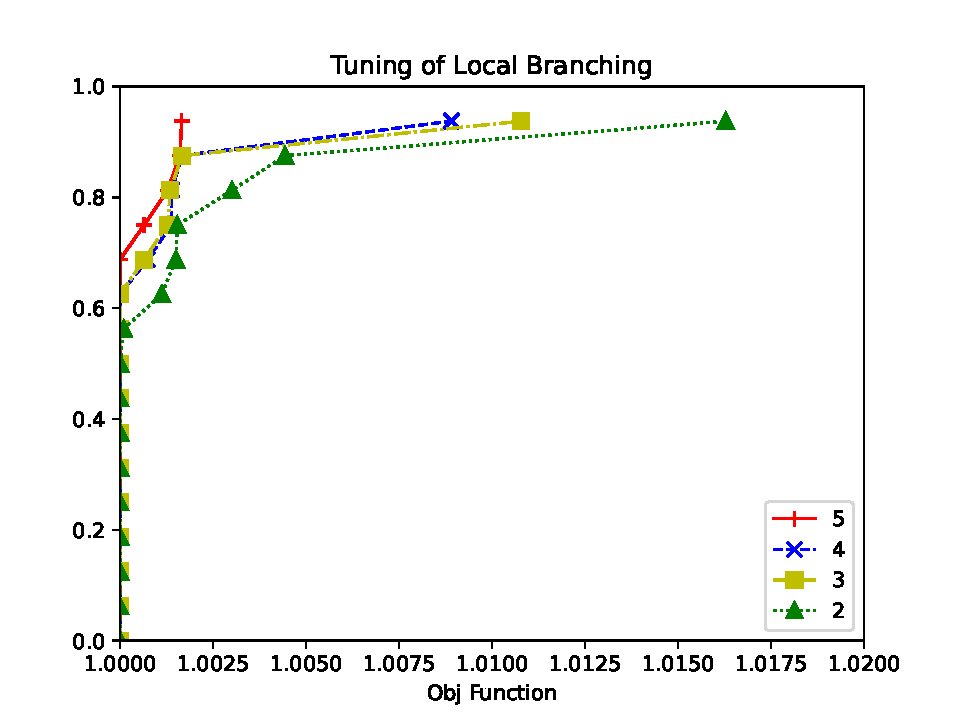
\includegraphics[width=\textwidth]{images/soft.pdf}
    \caption{Tuning of number of non improvement iteration before to change the value of k in Local Branching}
    \label{fig:soft}
\end{figure}


\section{Comparison of Matheuristics}

We tested the HardFixing Algorithm and the Local Branching Algorithm over the same instances, running for the same amount of time per instance. Both Figure \ref{fig:hs} and Table \ref{table:math} shows how they performs identically in more than 50\% of the instances, returning the same correct value. Overall HardFixing is by far the best one, since it provides stronger constraints and leads to more precise solutions. 

\begin{figure}[!h]
    \centering
    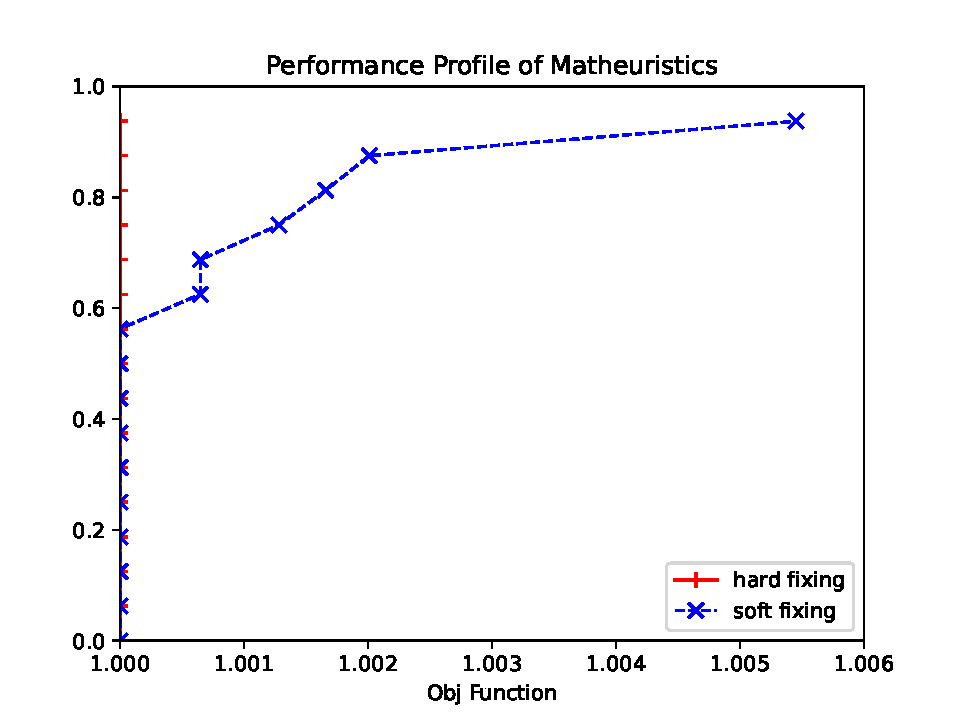
\includegraphics[width=\textwidth]{images/hs.pdf}
    \caption{Performance Profile of Matheuristics}
    \label{fig:hs}
\end{figure}

\begin{table}[!h]
    \centering
    \begin{tabular}{lcc}
    \cline{2-3}
                & \textbf{hard fixing} & \textbf{soft fixing} \\ \hline
    att48.tsp   & 10601.127450         & 10601.127450         \\
    att532.tsp  & 28212.391348         & 28248.540350         \\
    d493.tsp    & 35605.036596         & 35676.629322         \\
    d657.tsp    & 50855.493487         & 50855.493487         \\
    dsj1000.tsp & 21619342.0      & 21619342.0      \\
    lin318.tsp  & 42649.518313         & 42649.518313         \\
    p654.tsp    & 40251.581798         & 40251.581798         \\
    pcb442.tsp  & 51328.083821         & 51328.083821         \\
    pr1002.tsp  & 284653.597388        & 286205.676140        \\
    pr439.tsp   & 110741.414203        & 110741.414203        \\
    rat575.tsp  & 6960.514805          & 6965.028779          \\
    rat783.tsp  & 9307.311019          & 9322.754398          \\
    rd400.tsp   & 15516.720499         & 15516.720499         \\
    u574.tsp    & 38125.252074         & 38149.920552         \\
    u724.tsp    & 44201.295322         & 44201.295322         \\
    vm1084.tsp  & 276173.143915        & 276173.143915        \\ \hline
    \end{tabular}
    \caption{Results of Matheuristic Methods}
    \label{table:math}
    \end{table}

\clearpage{\pagestyle{plain}\cleardoublepage}
\chapter{Immagini e Tabelle} 
\label{chapter:immagini_e_tabelle} 
Metodi più comuni per inserire immagini e esempi di tabelle.

\section{Immagine singola}
Per fare riferimento ad un immagine, come ad ogni altro elemento a cui viene attribuita una \textit{label} è disponibile il comando \textit{ref}. Riferimento a Figura \ref{fig:figura_test}.
\begin{figure}[!h]
\centering

\includegraphics[scale=0.4]{images/test.png}
\caption{Didascalia}
\label{fig:figura_test}
\end{figure}

\section{Immagine multipla}
Inserire più ``sottofigure" in una figura.
\begin{figure}[!h]
\centering
	%Prima riga
	\begin{subfigure}{0.35\textwidth} %Controllo della posizione in orizzontale
		
\includegraphics[scale=0.15]{images/test.png} 
		\caption{}
	\end{subfigure}
	\begin{subfigure}{0.35\textwidth}
		
\includegraphics[scale=0.15]{images/test.png}
		\caption{}
	\end{subfigure}
	%Seconda riga
	\begin{subfigure}{0.35\textwidth}
		
\includegraphics[scale=0.15]{images/test.png} 
		\caption{}
	\end{subfigure}
	\begin{subfigure}{0.35\textwidth}
		
\includegraphics[scale=0.15]{images/test.png}
		\caption{}
	\end{subfigure}
\caption{Esempio di figura composta da 4 figure.}
\end{figure}

\section{Tabelle}
Nella seguente tabella vengono mostrati alcuni esempi di separazione delle righe. La separazione delle colonne avviene  all'interno delle parentesi grafe dopo il comando \textit{tabular}.
\begin{center}
\begin{tabular}{ ||c|c|c|| } 
 \hline
 cella1 & cella2 & cella3 \\
 \hline\hline 
 cella4 & cella5 & cella6 \\ 
 \hline
 cella7 & cella8 & cella9 \\ 
 cella10 & cella11 & cella12 \\ 
 \hline
\end{tabular}
\end{center}

È possibile, inoltre, fissare la dimensione delle colonne.

\begin{center}
\begin{tabular}{ | m{3cm} | m{5cm} | m{1.5cm} | } 
 \hline
 cella1 & cella2 & cella3 \\
 \hline\hline 
 cella4 & cella5 & cella6 cella6 cella6 cella6 \\ 
 \hline
 cella7 & cella8 & cella9 \\ 
 cella10 & cella11 & cella12 \\ 
 \hline
\end{tabular}
\end{center} 

\clearpage{\pagestyle{plain}\cleardoublepage}
\chapter{Formule} 
\label{chapter:formule} 
Per inserire delle formule matematiche è possibile utilizzare due metodi:
\begin{itemize}
\item in linea: inserendo la formula tra due caratteri \$. 
\item utilizzando l'ambiente \textit{equation}.
\end{itemize}

%Il comando noindent viene utilizzato per evitare l'indentazione del paragrafo
\noindent Esempio di formula in linea $x(t)=x_{0} + v_{0}t + \frac{1}{2}at^{2}$.

\noindent Esempio di utilizzo dell'ambiente \textit{equation}:
\begin{equation}\label{eq:legge_oraria}
x(t)=x_{0} + v_{0}t + \frac{1}{2}at^{2}
\end{equation}
Possiamo usare le \textit{label} anche per le equazioni. Legge oraria nell'Equazione \ref{eq:legge_oraria}.
Infine, un esempio di formula su più righe:
\begin{equation}
\begin{split}
x(t) &= x_{0} + v_{0}t + \frac{1}{2}at^{2} \\ & =
		x_{0} + v_{0}t + \frac{1}{2}\frac{F}{m}t^{2}
\end{split}
\end{equation} 

\clearpage{\pagestyle{plain}\cleardoublepage}
\chapter{Pseudocodice e codice} 
\label{chapter:codice} 
In questo template per l'inserimento di pseudocodice è stato utilizzato il pacchetto \textit{algpseudocode}. Per quanto riguarda l'inserimento del codice è possibile utilizzare il comando \textit{verb} per inserire in linea oppure \textit{lstlisting} per inserire blocchi di codice.

\section{Pseudocodice}
\begin{algorithm}
\caption{Nome algortimo}\label{algo:name}
\begin{algorithmic}[1]
\Require $\text{Input dell'algoritmo}$
\Ensure $\text{Output dell'algortimo}$
\State variabile $\gets$ assegnazione valore
\State valore\_ritornato $\gets$ \textsc{Funzione}\textsc{Prova}(param1, param2)

\For{\textit{element} in \textit{list}} 
\State res $\gets$ \textsc{Do}\textsc{Something}(element)
\EndFor

\If{condizione1}
\State do something

\ElsIf{condizione2}
\State do something else
\Else
\State \textbf{print} ``Hello World"
\EndIf
\end{algorithmic}
\end{algorithm}

\section{Codice}
È possibile inserire codice in linea: \verb!print("Hello World")!.\\
Inoltre è possibile usare l'ambiente \textit{lstlisting} configurando il layout del blocco di codice nel file \textit{layout.tex}. Il codice può essere importato da un file esterno che metteremo nella cartella \textit{code}.
\lstinputlisting[language=Python, caption=Didascalia., label=ls:codice]{code/randomized_search.py} 

\clearpage{\pagestyle{plain}\cleardoublepage}

\nocite{*}

%\begin{thebibliography}{99}
\addcontentsline{toc}{chapter}{Bibliografia}

\bibitem{sklearnArt}Buitinck L., Louppe G., Blondel M., Pedregosa F., Mueller A., Grisel O., Niculae V., Prettenhofer P., Gramfort A., Grobler J., Layton R., Vanderplas J., Joly A., Holt B., Varoquaux G., \textit{API design for machine learning software: Experiences from the scikit-learn project}, 2013. 

\bibitem{CNN} \textit{Convolutional Neural Networks}, \url{http://deeplearning.net/tutorial/ lenet.html}, last consultation: 07/01/2020.

\end{thebibliography}


\bibliographystyle{plain} % We choose the "plain" reference style
\bibliography{biblio.bib} % Entries are in the refs.bib file
\end{document}
